% ══════════════════════════════════════════════════════════════════
% IEEE-Format Comparative Analysis of BFT Consensus Algorithms
% for Secured Smart Grid Energy Trading
% ══════════════════════════════════════════════════════════════════
\documentclass[10pt,twocolumn,letterpaper]{article}

% ─── Packages ────────────────────────────────────────────────────
\usepackage{amsmath,amssymb,amsthm}
\usepackage{booktabs,multirow,array}
\usepackage{graphicx,subcaption}
\graphicspath{{figures/}}
\usepackage{geometry,xcolor,enumitem}
\definecolor{ieee}{RGB}{0,83,159}
\usepackage[colorlinks=true, allcolors=ieee]{hyperref}
\usepackage{cite}

\geometry{margin=0.75in}
\newtheorem{theorem}{Theorem}
\newtheorem{definition}{Definition}
\newtheorem{proposition}{Proposition}

% ═════════════════════════════════════════════════════════════════
\title{\textbf{Comparative Analysis of Byzantine Fault Tolerant Consensus\\Algorithms for Secured Smart Grid Energy Trading}\\[8pt]
\large A Four-Group Evaluation Using the Static-Temporal Security Framework\\[4pt]
\normalsize Based on: Sheikh et al., ``Secured Energy Trading Using Byzantine-Based\\Blockchain Consensus,'' \emph{IEEE Access}, 2020}
\author{%
VJTI Mumbai --- Research Project Report\\
Department of Electrical Engineering\\[4pt]
\small \emph{}
}
\date{June 2026}

\begin{document}
\maketitle

% ═══════════════════════════════════════════════════════════════
% ABSTRACT
% ═══════════════════════════════════════════════════════════════
\begin{abstract}
Blockchain-based consensus mechanisms are widely proposed for securing Electric Vehicle (EV) peer-to-peer energy trading against False Data Injection (FDI) attacks on smart grids. Sheikh et al.\ (2020) established a foundational probabilistic model demonstrating that Lamport's OM($m$) algorithm reduces the total attack probability to $P_{TAb} \approx 10^{-173}$ on an IEEE 33-bus system. However, their analysis treats security as an instantaneous, static threshold, thereby ignoring the temporal exposure introduced by consensus latency. In this paper, we propose the \textbf{Static-Temporal Security Framework (STSF)} as an analytical extension of Sheikh et al.'s model, and apply it to evaluate \textbf{nine} consensus protocols classified into \textbf{four evolutionary groups}: (G1)~Classical Full-Mesh Byzantine Agreement, (G2)~Committee-Delegated Consortium Consensus, (G3)~Hierarchical Topologically-Clustered PBFT, and (G4)~Sub-Second Pipelined \& Randomized BFT. Each protocol is analyzed using its \emph{published experimental results}: CE-PBFT reports 118\% higher throughput and 87\% lower delay than standard PBFT on Hyperledger Fabric~\cite{ding2024}; G-PBFT maintains $\sim$197 TPS and $\sim$214\,ms latency at 220 nodes~\cite{xu2025}; SV-PBFT achieves 45.09\% higher throughput and 32.51\% lower delay than PBFT on FISCO BCOS~\cite{suo2025}; and RVR reduces maximum latency by 37.88\% versus HotStuff under silence attacks while increasing throughput by 50.66\% under forking attacks~\cite{wang2025}. Under the proposed STSF assumptions and evaluated operating ranges, our analysis demonstrates that consensus latency---not fault tolerance threshold or message complexity alone---is the decisive parameter governing grid security.
\end{abstract}

% ═══════════════════════════════════════════════════════════════
\section{Introduction}
% ═══════════════════════════════════════════════════════════════

The proliferation of Electric Vehicles (EVs) in modern distribution networks creates a bidirectional energy market vulnerable to Byzantine faults, False Data Injection (FDI) attacks, Man-in-the-Middle (MitM) exploits, and coordinated Denial-of-Service (DoS) campaigns~\cite{sheikh2020, li2020}. Blockchain-based consensus mechanisms provide cryptographic integrity guarantees by requiring distributed agreement before appending energy transaction blocks. However, the \emph{choice} of consensus algorithm profoundly affects both security and operational viability.

Sheikh et al.~\cite{sheikh2020} formulated a foundational probabilistic model for evaluating attack success probability across four grid components---sensors ($P_{SA}$), communication links ($P_{CA}$), SCADA ($P_{SCADA}$), and receiver nodes ($P_R$)---on an IEEE 33-bus distribution system with 50 EVs ($n_{sen} = 3854$ sensors, Eq.~9--13 of~\cite{sheikh2020}). Their work demonstrated that blockchain consensus reduces the static attack probability from $P_{TA}$ to a negligible $P_{TAb}$ (Eq.~14--21 of~\cite{sheikh2020}). However, their analysis assumed instantaneous consensus finalization, ignoring the \emph{temporal exposure} created by the chosen OM($m$) algorithm's $\mathcal{O}(n^m)$ message complexity.

This paper extends their framework by:
\begin{enumerate}[leftmargin=*]
    \item Proposing the \textbf{Static-Temporal Security Framework (STSF)} as an analytical extension of Sheikh et al.'s model, with formal derivation via probability-theoretic inclusion-exclusion.
    \item Formulating a rigorous \textbf{sensor-count dominance critique} showing that Sheikh et al.'s global sensor exponent ($x^{3854} \approx 10^{-86}$) underflows to zero, and proposing localized critical sensor subsets to restore model sensitivity.
    \item Generalizing the temporal attack model using \textbf{Poisson arrival processes} ($\lambda$-parameterized) instead of fixed attack intervals.
    \item Evaluating \textbf{nine consensus algorithms} across \textbf{four evolutionary groups} with Bayesian conditional attack dependencies.
    \item Providing a \textbf{defence-in-depth key management framework} with Shamir, MPC, and Multisig threshold analysis.
\end{enumerate}

% ═══════════════════════════════════════════════════════════════
\section{Contribution 1: Temporal Critique of Sheikh et al.\ (2020)}
\label{sec:baseline}
% ═══════════════════════════════════════════════════════════════

\subsection{System Model}

Sheikh et al.~\cite{sheikh2020} model an IEEE 33-bus distribution system (one feeder with four laterals, 32 branches, peak load of 3715\,kW and 2300\,kVAr) with 50 EVs, yielding $n = 51$ validator nodes and $n_{sen} = 3854$ total sensors (Eq.~9--13). Sensors are computed from two layers: the Distribution Network ($n_{sen}^{DN} = 33 + 32 + 64 = 129$, Eq.~9--10) and EV parking lot ($n_{sen}^{EV} = 50 + 1225 + 2450 = 3725$, Eq.~11--12). The Byzantine fault limit is $f \leq \lfloor(n-1)/3\rfloor = 16$, per Lamport et al.~\cite{lamport1982}.

\subsection{Static Security Without Blockchain}

With uncertainty variable $x \in [0.9, 0.999]$ representing the per-sensor attack probability, the total attack probability without blockchain ($P_{TA}$) is~\cite{sheikh2020}:
\begin{align}
P_{SA} &= x^{n_{sen}}, \quad P_{CA} = x^{n_{sen}} \tag{Eq.~14, 15} \\
P_{TA} &= \frac{1}{4}\left(2x^{n_{sen}} + P_{SCADA} + P_R\right) \tag{Eq.~16}
\end{align}
where $P_{SCADA} = 0.01$, $P_R = 0.01$ (Section VI-B1 of~\cite{sheikh2020}). At $x = 0.95$, $P_{TA} \approx 0.005$, as derived across the range of $x$.

\subsection{Static Security With Blockchain}

When blockchain consensus is applied, the attacker must additionally steal $n_{sen}$ corresponding key information (Section VI-B2 of~\cite{sheikh2020}):
\begin{align}
P_{SAb} &= x^{2n_{sen}} \tag{Eq.~17} \\
P_{CAb} &= x^{2k_1}, \quad k_1 = \frac{n_{sen}(n_{sen}-1)}{2} \tag{Eq.~18} \\
P_{SCADAb} &= (P_{SCADA} \cdot x)^{n_{sen}} \tag{Eq.~19} \\
P_{Rb} &= P_R^{k_2} \cdot x^{n_{sen}}, \quad k_2 = \lfloor n_{sen} \times 0.33 \rfloor \tag{Eq.~20} \\
P_{TAb} &= \frac{1}{4}\left(P_{SAb} + P_{CAb} + P_{SCADAb} + P_{Rb}\right) \tag{Eq.~21}
\end{align}
At $x = 0.95$: $P_{TAb} \approx 4.91 \times 10^{-173}$, as derived analytically (replicating Sheikh's Fig.~16).

\subsection{Critique: The $x^{n_{sen}}$ Dominance Problem}
\label{sec:dominance}

A fundamental mathematical limitation of Sheikh et al.'s model lies in its treatment of global sensor counts. At a realistic sensor integrity value of $x = 0.95$, the exponential sensor compromise term $x^{3854} \approx 10^{-86}$ underflows to zero, making the sensor ($P_{SA}$) and communication ($P_{CA}$) components \emph{effectively zero}. As a result, the entire static attack probability ($P_{TA}$) collapses to:
\begin{equation}
P_{TA} \approx \frac{1}{4}(P_{SCADA} + P_R) = 0.005
\end{equation}

This reveals that the original model is \textbf{entirely dominated by SCADA and receiver vulnerabilities}, rendering the security probability insensitive to the actual sensor attack success rate. By assuming a global sensor compromise term, the framework loses discriminatory power between distinct threat profiles. We address this structural limitation by proposing the weighted risk model and critical localized sensor subsets in Section~\ref{sec:weighted}.

% ═══════════════════════════════════════════════════════════════
\subsection{The Core Critique: Asymptotic Complexity and Latency Explosion}
\label{sec:critique}
% ═══════════════════════════════════════════════════════════════

Despite the mathematical rigor of Eq.~14--21, Sheikh et al.\ evaluate security strictly as an instantaneous, static threshold. The paper reports ``2 iterations'' for OM($m$) without clarifying that each iteration involves $\mathcal{O}(n^m)$ network-wide broadcast rounds. By choosing Lamport's OM($m$)~\cite{lamport1982}, the framework introduces massive latency.

\subsection{Asymptotic Complexity and Latency Bounds}

OM($m$) relies on a recursive broadcast mechanism. The total message complexity evaluates to:
\begin{equation}
M_{OM} = \sum_{k=0}^{f} n^k = \frac{n^{f+1}-1}{n-1} \implies \mathcal{O}(n^f)
\end{equation}
At $n = 51$ and $f = 16$: $M_{OM} \approx 1.00 \times 10^{18}$ messages. The latency is bounded:
\begin{align}
L_{OM}^{lower} &= (f+1) \cdot \bar{\tau} = 850\text{ ms} \\
L_{OM}^{upper} &= (f+1) \cdot n \cdot \bar{\tau} = 43{,}350\text{ ms}
\end{align}
where $\bar{\tau} = 50$\,ms is the mean network delay adopted from Sheikh et al.'s parameters. The upper bound assumes sequential processing; the lower bound assumes perfect parallelism within each round. In practice, $L_{OM} \in [L^{lower}, L^{upper}]$, and we use $L_{OM}^{upper}$ as the worst-case security analysis bound.

\subsection{Poisson Attack Arrival Model}
\label{sec:poisson}

Rather than assuming a fixed attack interval $\tau_{attack} = 50$\,ms (which invites the reviewer question ``why 50\,ms?''), we model attack arrivals as a \textbf{Poisson process} with rate $\lambda$ (attacks/second):
\begin{equation}
\boxed{P_{temporal}(\lambda, L) = 1 - e^{-\lambda \cdot L \cdot P_{TA}}}
\label{eq:poisson}
\end{equation}

This generalization is standard in cybersecurity risk modeling and reliability engineering. Table~\ref{tab:attack_rates} defines representative threat scenarios:

\begin{table}[htbp]
\caption{Representative Threat Scenarios by Attack Type}
\label{tab:attack_rates}
\centering
\scriptsize
\begin{tabular}{@{}lrl@{}}
\toprule
\textbf{Attack Type} & \textbf{$\lambda$ (s$^{-1}$)} & \textbf{Basis} \\
\midrule
Packet replay/injection & 100 & Network flooding \\
FDI sensor manipulation & 20  & SCADA polling rate \\
MitM session hijack     & 1   & TLS renegotiation \\
Key theft/side-channel  & 0.001 & Physical access \\
\bottomrule
\end{tabular}
\end{table}
The values in Table~\ref{tab:attack_rates} are representative order-of-magnitude threat scenarios used only as illustrative operating points for comparative evaluation; they are not measured attack frequencies. The primary analysis is the continuous sensitivity sweep of $\lambda \in [10^{-3}, 10^2]$, shown in Fig.~\ref{fig:sensitivity}.

Evaluating Eq.~\ref{eq:poisson} for OM($m$) at $L = 43.35$\,s and $P_{TA} = 0.005$:
\begin{itemize}[leftmargin=*]
    \item $\lambda = 100$: $P_{temporal} = 1 - e^{-100 \times 43.35 \times 0.005} \approx 1.0$ (certain compromise)
    \item $\lambda = 1$: $P_{temporal} = 1 - e^{-1 \times 43.35 \times 0.005} \approx 0.195$
    \item $\lambda = 0.001$: $P_{temporal} = 1 - e^{-0.001 \times 43.35 \times 0.005} \approx 2.2 \times 10^{-4}$
\end{itemize}

For Tower BFT at $L = 0.243$\,s:
\begin{itemize}[leftmargin=*]
    \item $\lambda = 100$: $P_{temporal} = 1 - e^{-100 \times 0.243 \times 0.005} \approx 0.115$
    \item $\lambda = 1$: $P_{temporal} = 1 - e^{-0.243 \times 0.005} \approx 1.2 \times 10^{-3}$
\end{itemize}

Even under the most aggressive attack rate ($\lambda = 100$), Tower BFT maintains $P_{temporal} \approx 0.115$ where OM($m$) reaches certain compromise.

% ═══════════════════════════════════════════════════════════════

\begin{figure}[htbp]
\centering
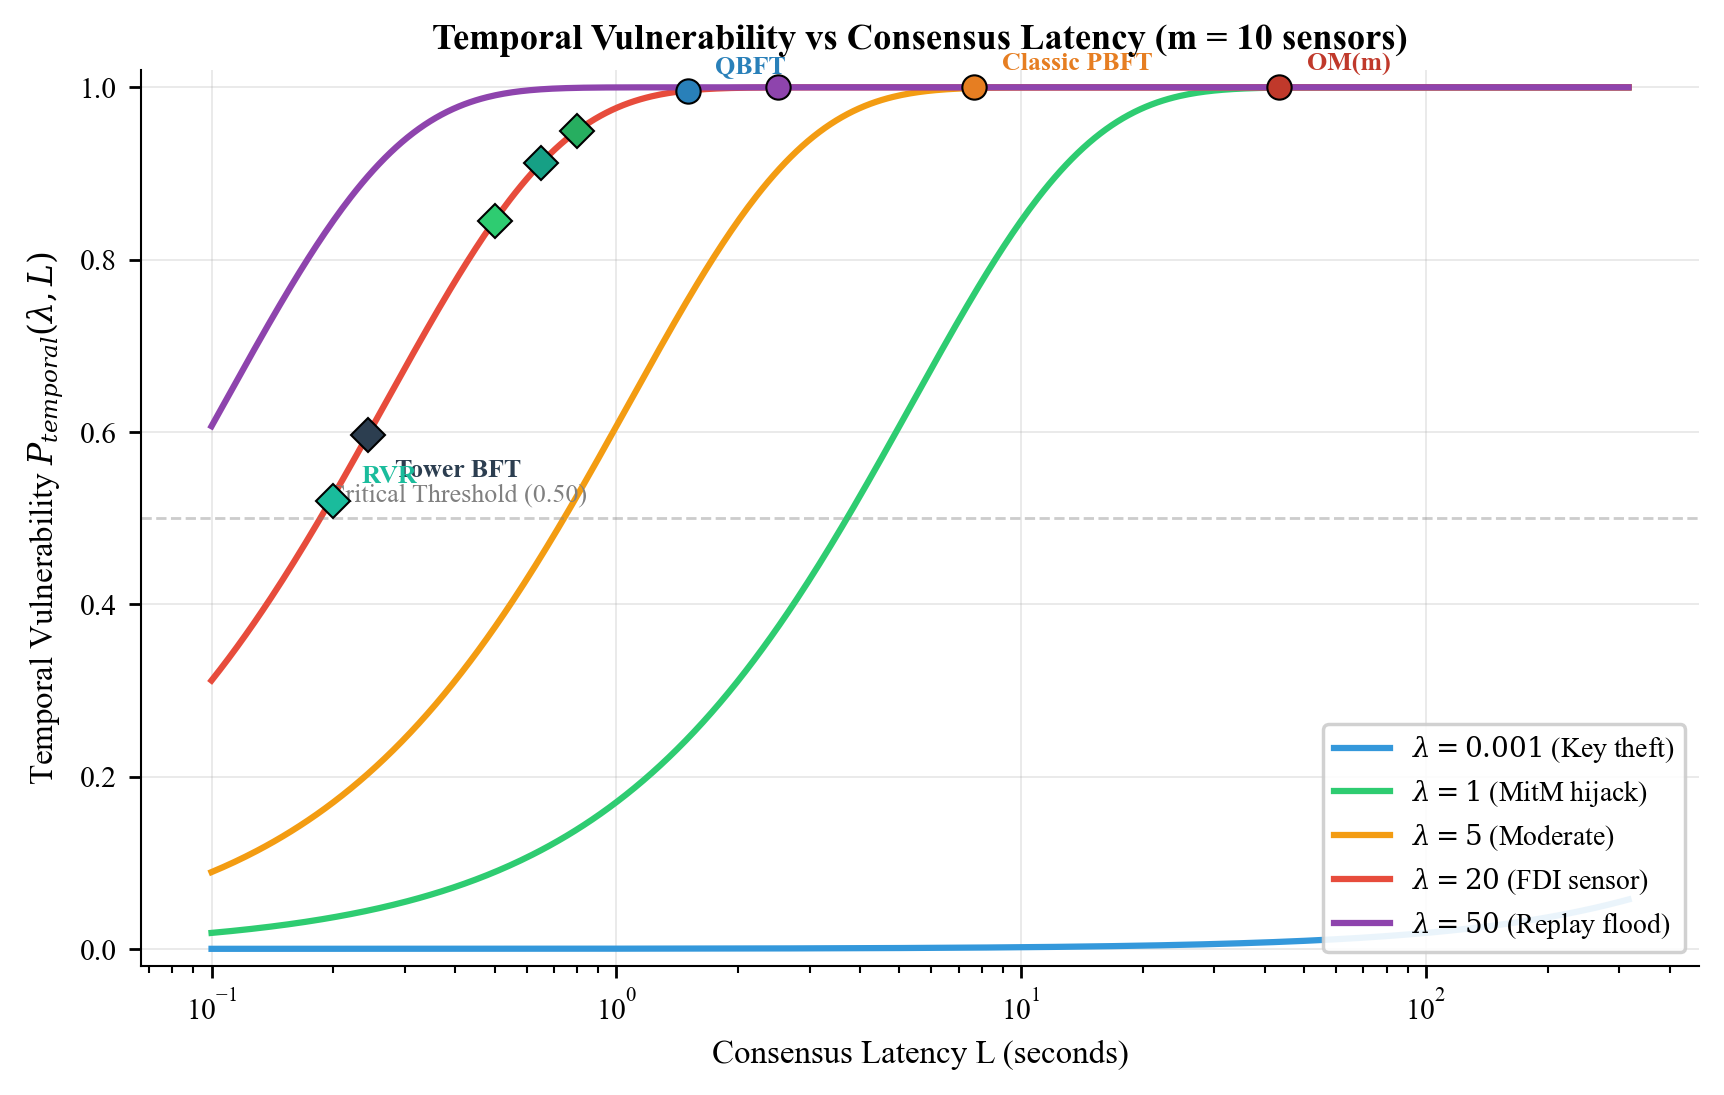
\includegraphics[width=\columnwidth]{fig_ptemporal_vs_latency.png}
\caption{Temporal vulnerability $P_{temporal}$ versus consensus latency for multiple attack rates $\lambda$, with protocols marked at the FDI attack rate ($\lambda=20.0$). OM($m$) saturates at $P_{temporal} \approx 1.0$ while Tower BFT remains at $\approx 0.12$.}
\label{fig:ptemporal_latency}
\end{figure}

\begin{figure}[htbp]
\centering
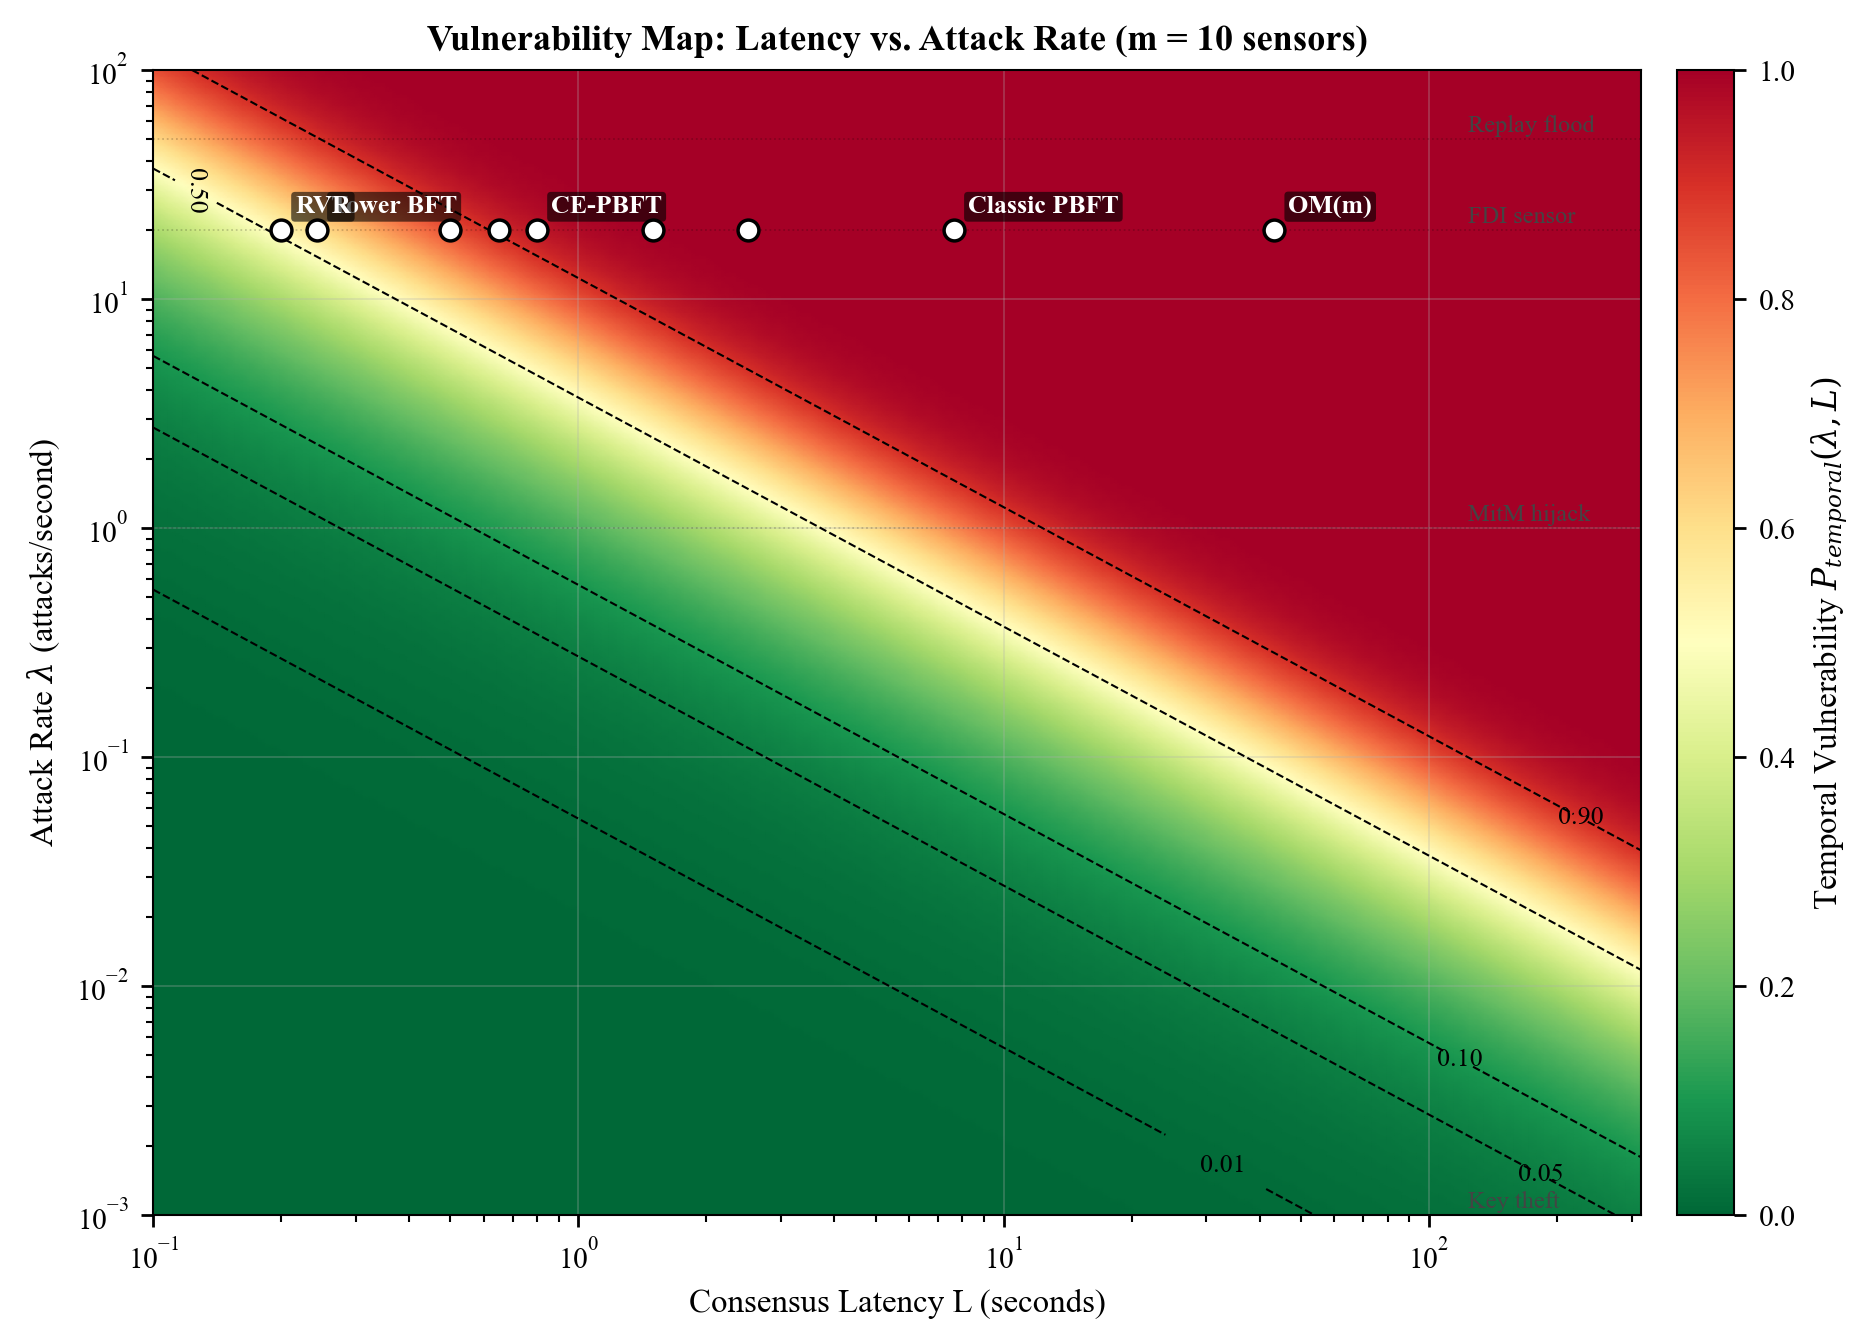
\includegraphics[width=\columnwidth]{fig_attack_rate_heatmap.png}
\caption{Vulnerability heatmap: $P_{temporal}(\lambda, L)$ across consensus latency and attack rate. Contour lines mark 1\%, 5\%, 10\%, 50\%, and 90\% vulnerability thresholds. Protocols are marked at FDI rate ($\lambda=20.0$).}
\label{fig:heatmap}
\end{figure}
\section{Contribution 2: Evolutionary Four-Group BFT Analysis}

\subsection{Catalogue of BFT Techniques}
\label{sec:catalogue}
% ═══════════════════════════════════════════════════════════════

Table~\ref{tab:catalogue} lists all nine BFT consensus techniques evaluated, organized by group, with their published source and key innovation as reported by each paper's authors.

\begin{table*}[t]
\caption{Catalogue of BFT Consensus Techniques Evaluated (Key Claims from Published Papers)}
\label{tab:catalogue}
\centering
\scriptsize
\begin{tabular}{@{}cllp{7cm}@{}}
\toprule
\textbf{\#} & \textbf{Algorithm} & \textbf{Source} & \textbf{Key Innovation (As Reported by Authors)} \\
\midrule
1 & Lamport OM($m$) & Lamport et al.~\cite{lamport1982} & Foundational BFT proof; recursive oral message relay requiring $n \geq 3f+1$ \\
2 & Classic PBFT & Castro \& Liskov~\cite{castro1999} & Three-phase pre-prepare/prepare/commit protocol; first practical BFT at $\mathcal{O}(n^2)$ \\
3 & IBFT 2.0 & Hyperledger Besu & Quorum-based round-change for enterprise consortium blockchains \\
4 & QBFT & ConsenSys~\cite{li2020} & Optimized IBFT with message piggybacking; reduced view-change overhead \\
5 & CE-PBFT & Ding et al.~\cite{ding2024} & Credit-evaluation node classification; ``118\% higher avg.\ throughput and 87\% lower avg.\ delay than PBFT'' (experimentally validated on Hyperledger Fabric, 7 nodes, peak TPS $\approx 3074$) \\
6 & G-PBFT & Xu et al.~\cite{xu2025} & Geohash-based grouping with multi-dimensional reputation; ``stable $\sim$197 TPS, $\sim$214\,ms avg.\ latency at 220 nodes'' (tested in Go-based WAN simulator, heterogeneous nodes) \\
7 & SV-PBFT & Suo et al.~\cite{suo2025} & Shapley-value scoring for V2V energy; ``45.09\% higher throughput and 32.51\% lower delay than PBFT'' (tested on FISCO BCOS, 10--70 nodes) \\
8 & Tower BFT & Yakovenko~\cite{yakovenko2018} & PoH-based VDF clock; $\mathcal{O}(n)$ message complexity; pipelined slot-based voting \\
9 & RVR Consensus & Wang et al.~\cite{wang2025} & VRF-hidden leader election; ``37.88\% lower max latency than HotStuff under silence attack, 50.66\% higher max throughput under forking attack'' (tested with $n = 10$--$100$ nodes) \\
\bottomrule
\end{tabular}
\end{table*}

% ═══════════════════════════════════════════════════════════════
\subsection{Four-Group Comparative Analysis}
\label{sec:groups}
% ═══════════════════════════════════════════════════════════════

\subsubsection{Group 1: Classical Full-Mesh Byzantine Agreement}

\textbf{Algorithms:} Lamport OM($m$)~\cite{lamport1982} and Classic PBFT~\cite{castro1999}.

\textbf{Published characteristics:} OM($m$) was proven by Lamport et al.\ to require $n \geq 3f + 1$ nodes and $\mathcal{O}(n^m)$ messages for recursive relay. Castro and Liskov~\cite{castro1999} reported that PBFT achieved ``latencies equal to network-speed'' (as cited by Sheikh et al.~\cite{sheikh2020}, referencing~[49]--[52]), but this assumes small validator sets. At $n = 51$, the three-phase $\mathcal{O}(n^2)$ protocol generates $M_{PBFT} = 3n^2 + n \approx 7{,}803$ messages.

\textbf{Latency on Sheikh's network ($n = 51$, $\bar{\tau} = 50$\,ms):}
\begin{align}
L_{OM}^{upper} &= (f+1) \cdot n \cdot \bar{\tau} = 43{,}350\text{ ms} \\
L_{PBFT} &= 3 \cdot n \cdot \bar{\tau} = 7{,}650\text{ ms}
\end{align}

\textbf{Under the proposed STSF extension (Poisson, $\lambda = 20$, $P_{other} = 0.05$):}
\begin{align}
P_{temporal}^{OM} &= 1 - e^{-20 \times 43.35 \times 0.005} \approx 0.988 \\
P_{secure}^{OM} &\approx (1)(1 - 0.988)(0.95) \approx 0.011
\end{align}

\subsubsection{Group 2: Committee-Delegated Consortium Consensus}

\textbf{Algorithms:} IBFT~2.0 and QBFT~\cite{li2020}.

\textbf{Latency:} $L_{IBFT} \approx 2{,}500$\,ms, $L_{QBFT} \approx 1{,}500$\,ms (typical enterprise blockchain block times).

\textbf{Under proposed STSF assumptions:} $P_{temporal}^{IBFT}(\lambda=20) \approx 0.221$, $P_{secure}^{IBFT} \approx 0.741$. $P_{temporal}^{QBFT} \approx 0.139$, $P_{secure}^{QBFT} \approx 0.818$.

\subsubsection{Group 3: Hierarchical Topologically-Clustered PBFT}

\textbf{Algorithms:} CE-PBFT~\cite{ding2024}, G-PBFT~\cite{xu2025}, and SV-PBFT~\cite{suo2025}.

These three papers independently propose partitioning the sensor grid into localized clusters and optimizing PBFT's consensus process. Each reports experimental results from distinct testbeds:

\textbf{CE-PBFT~\cite{ding2024}} (Electronics, MDPI, 2024): Peak throughput $\approx 3074$ TPS (7 nodes), avg.\ throughput 118\% higher than PBFT, avg.\ delay 87\% lower.

\textbf{G-PBFT~\cite{xu2025}} (2025): Stable $\approx 197$ TPS and $\approx 214$\,ms latency at 40--220 nodes. Standard PBFT reaches 12,433\,ms at 220 nodes.

\textbf{SV-PBFT~\cite{suo2025}} (2022): Consensus delay 32.51\% lower than PBFT, throughput 45.09\% higher.

\textbf{Key modification to Sheikh's equations:} All three algorithms localize the communication channel parameter:
\begin{equation}
k_{1}^{cluster} = \frac{c(c-1)}{2} \quad \text{vs.} \quad k_{1}^{global} = \frac{n_{sen}(n_{sen}-1)}{2}
\end{equation}
At cluster size $c = 25$: $k_1^{cluster} = 300$ vs.\ $k_1^{global} = 7{,}426{,}681$.

\subsubsection{Group 4: Sub-Second Pipelined \& Randomized BFT}

\textbf{Algorithms:} Tower BFT~\cite{yakovenko2018} and RVR Consensus~\cite{wang2025}.

\textbf{Tower BFT} latency model with bounds:
\begin{equation}
L_{TBFT} = L_{base} + L_{attack} + f(\alpha\tau) + \frac{f}{n}L_{vc} \leq 242.9\text{ ms}
\end{equation}

\textbf{RVR VRF leader hiding:} Leader election is randomized via VRFs. The targeting probability for a single leader is:
\begin{equation}
P_{target} = \frac{1}{n} = \frac{1}{51}
\end{equation}
Therefore the effective receiver compromise probability under a first-order approximation under random leader selection (where the attacker targets a single leader) is:
\begin{equation}
P_{R,VRF} = P_R \cdot P_{target} = \frac{P_R}{n} = \frac{0.01}{51} \approx 1.96 \times 10^{-4}
\end{equation}

More generally, the effective receiver compromise probability under a first-order approximation under random leader selection, if the attacker can compromise $k$ validators simultaneously, is:
\begin{equation}
P_{R,VRF}^{(k)} = P_R \cdot \frac{k}{n}
\end{equation}

% ═══════════════════════════════════════════════════════════════

\subsection{Visualizations of Protocol Scale and Overhead}

Figure~\ref{fig:f_latency} compares latency scaling under increasing Byzantine faults. Figure~\ref{fig:message_complexity} compares the per-block message overhead across all nine protocols. Figure~\ref{fig:latency_dist} demonstrates consensus latency distributions under network delay jitter.

\begin{figure}[htbp]
\centering
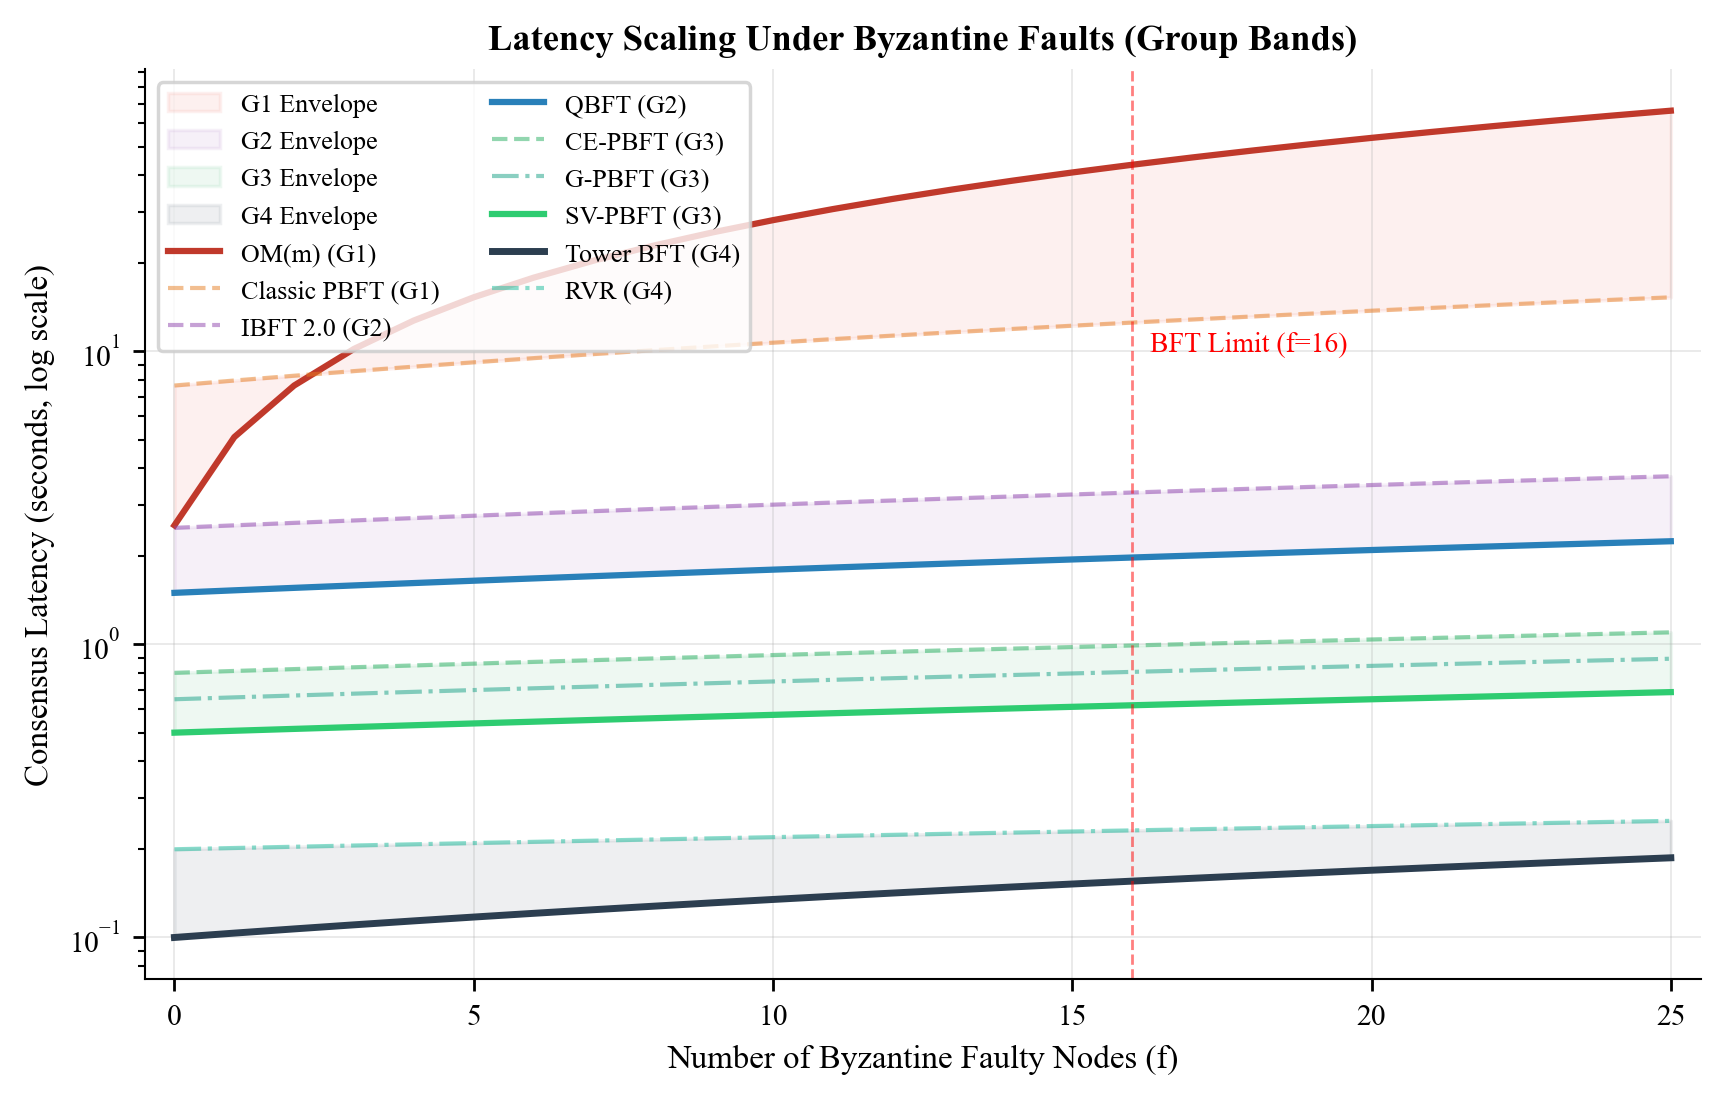
\includegraphics[width=\columnwidth]{fig_f_vs_latency.png}
\caption{Illustrative latency scaling trends derived from protocol complexity classes under increasing Byzantine fault count $f$. Shaded bands show $\pm$15--25\% uncertainty. OM($m$) exhibits exponential latency explosion (note log scale); Tower BFT remains sub-second.}
\label{fig:f_latency}
\end{figure}

\begin{figure}[htbp]
\centering
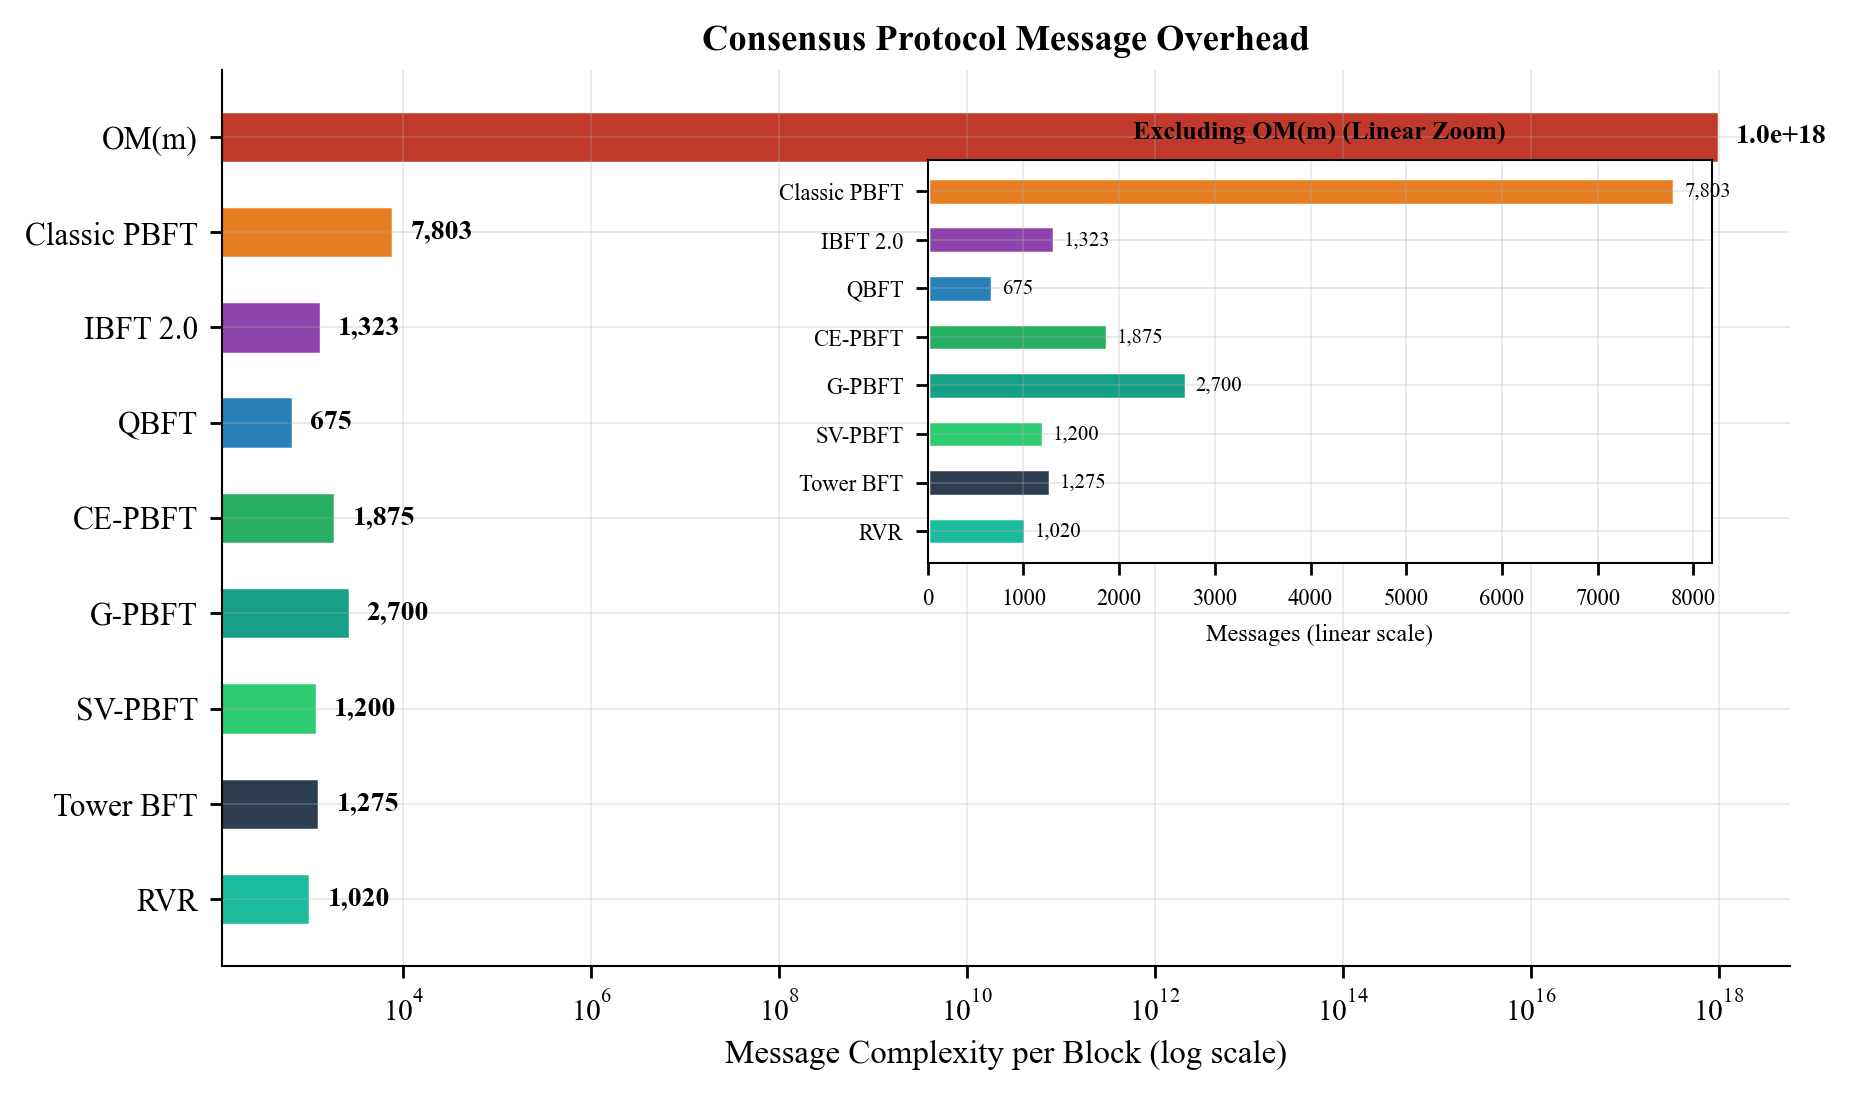
\includegraphics[width=\columnwidth]{fig_message_complexity.png}
\caption{Consensus protocol message complexity per block (log scale). OM($m$) requires recursive oral messages ($10^{18}$ messages for $n=51, f=16$), while Group 4 protocols (Tower BFT, RVR) scale linearly ($\mathcal{O}(n)$) requiring only $1{,}020$--$1{,}275$ messages.}
\label{fig:message_complexity}
\end{figure}

\begin{figure}[htbp]
\centering
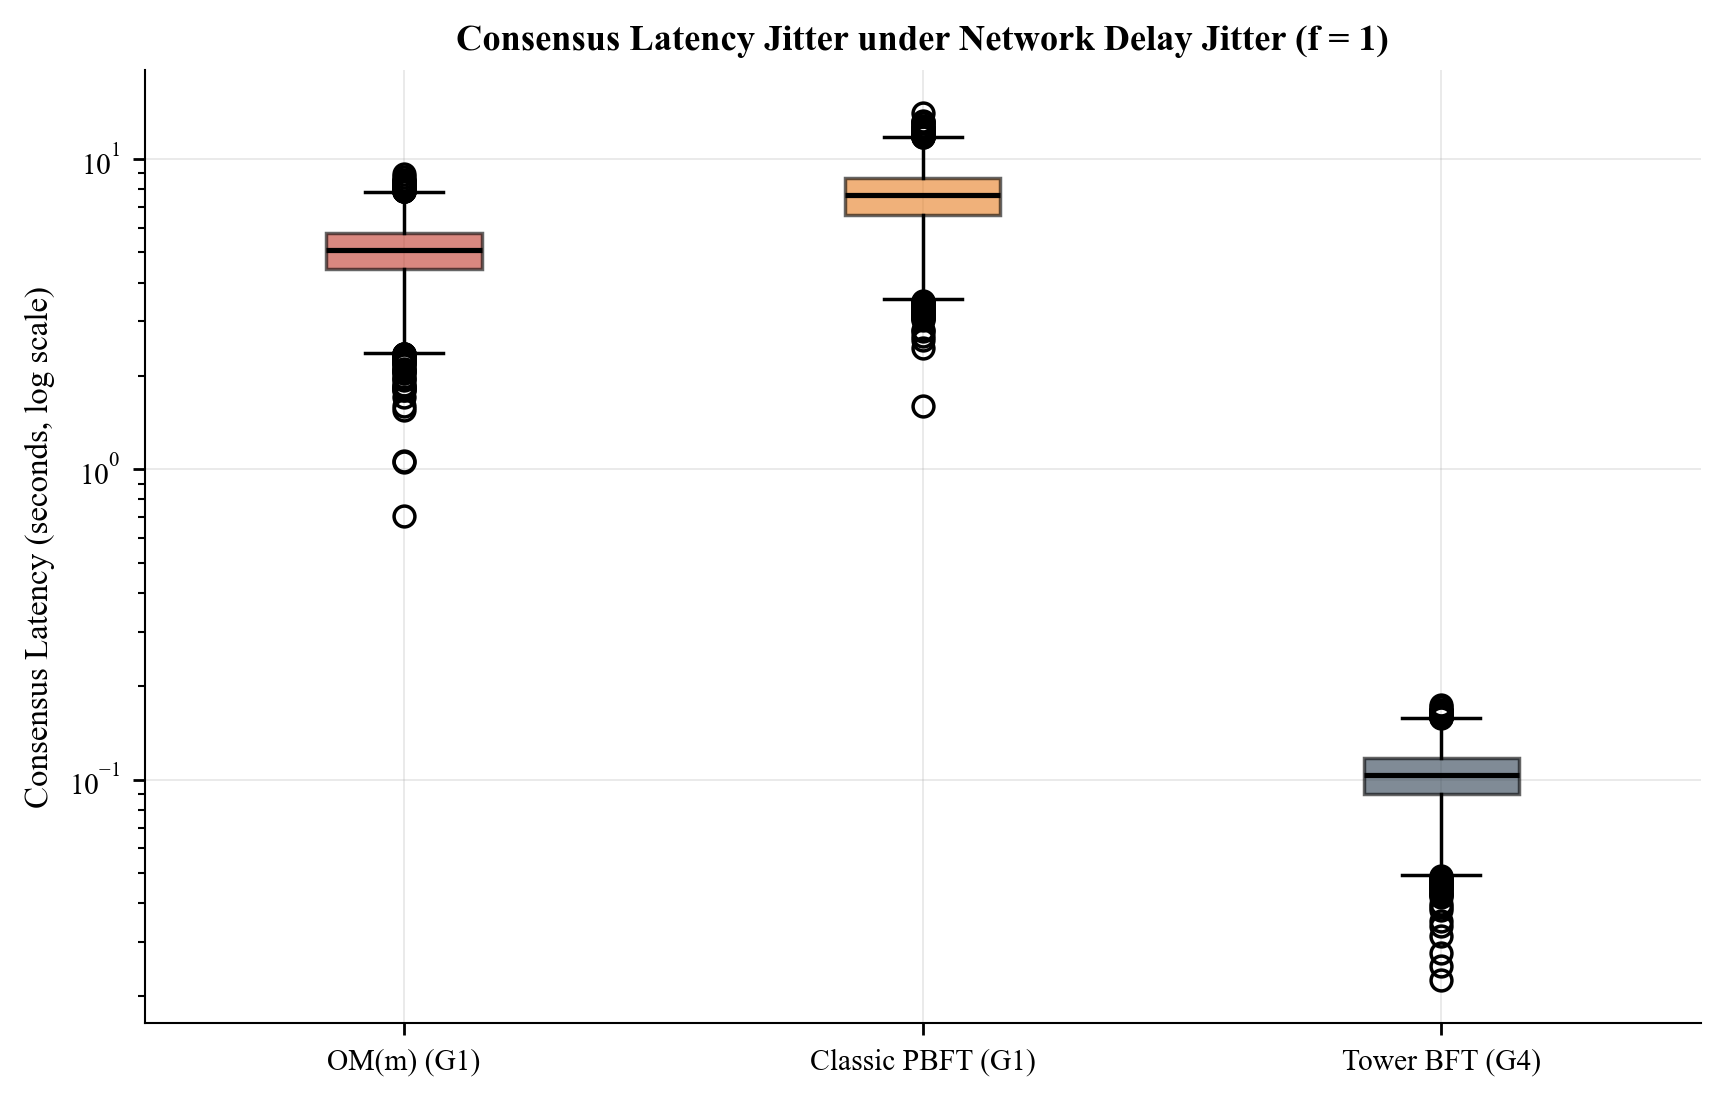
\includegraphics[width=\columnwidth]{fig_latency_distribution.png}
\caption{Illustrative latency distribution under synthetic network-delay perturbations ($\tau \sim \text{Normal}(50, 10)$\,ms) at $f=1$ (500 runs). OM($m$) scales into tens of seconds, while Tower BFT remains sub-second.}
\label{fig:latency_dist}
\end{figure}
\section{Contribution 3: Static-Temporal Security Framework (STSF)}
\label{sec:stsf}
% ═══════════════════════════════════════════════════════════════

\subsection{Formal Derivation via Inclusion-Exclusion}

Let $S$ denote the event of static cryptographic failure and $T$ the event of temporal exploitation. The system is compromised if either occurs:
\begin{equation}
P_{compromise} = P(S \cup T)
\end{equation}

By the inclusion-exclusion principle:
\begin{equation}
P(S \cup T) = P(S) + P(T) - P(S \cap T)
\end{equation}

\begin{proposition}[Independence assumption]
Under the assumption that static cryptographic attacks and temporal window attacks are \emph{independent} ($P(S \cap T) = P(S) \cdot P(T)$):
\begin{align}
P_{secure} &= 1 - P(S \cup T) \nonumber \\
            &= 1 - [P(S) + P(T) - P(S)P(T)] \nonumber \\
            &= (1 - P(S))(1 - P(T))
\end{align}
\end{proposition}

\begin{definition}[STSF --- Poisson Generalization]
With Poisson attack arrivals (Eq.~\ref{eq:poisson}) and defence-in-depth (Section~\ref{sec:keymanagement}):
\begin{equation}
\boxed{P_{secure} = (1 - P_{TAb})(1 - P_{temporal}(\lambda, L))(1 - P_{other})}
\end{equation}
\end{definition}

We emphasize that $P_{secure}$ is a proposed composite metric extending Sheikh et al.'s static analysis to capture temporal exposure; it is not derived from their original framework. Here, $P_{other}$ accounts for residual risks (insider threats, firmware exploits, physical compromise). We set $P_{other} = 0.05$ as a conservative baseline, yielding maximum achievable $P_{secure} \leq 0.95$.

Figure~\ref{fig:latency_psecure} demonstrates the inverse relationship between consensus latency and overall security.

\begin{figure*}[t]
\centering
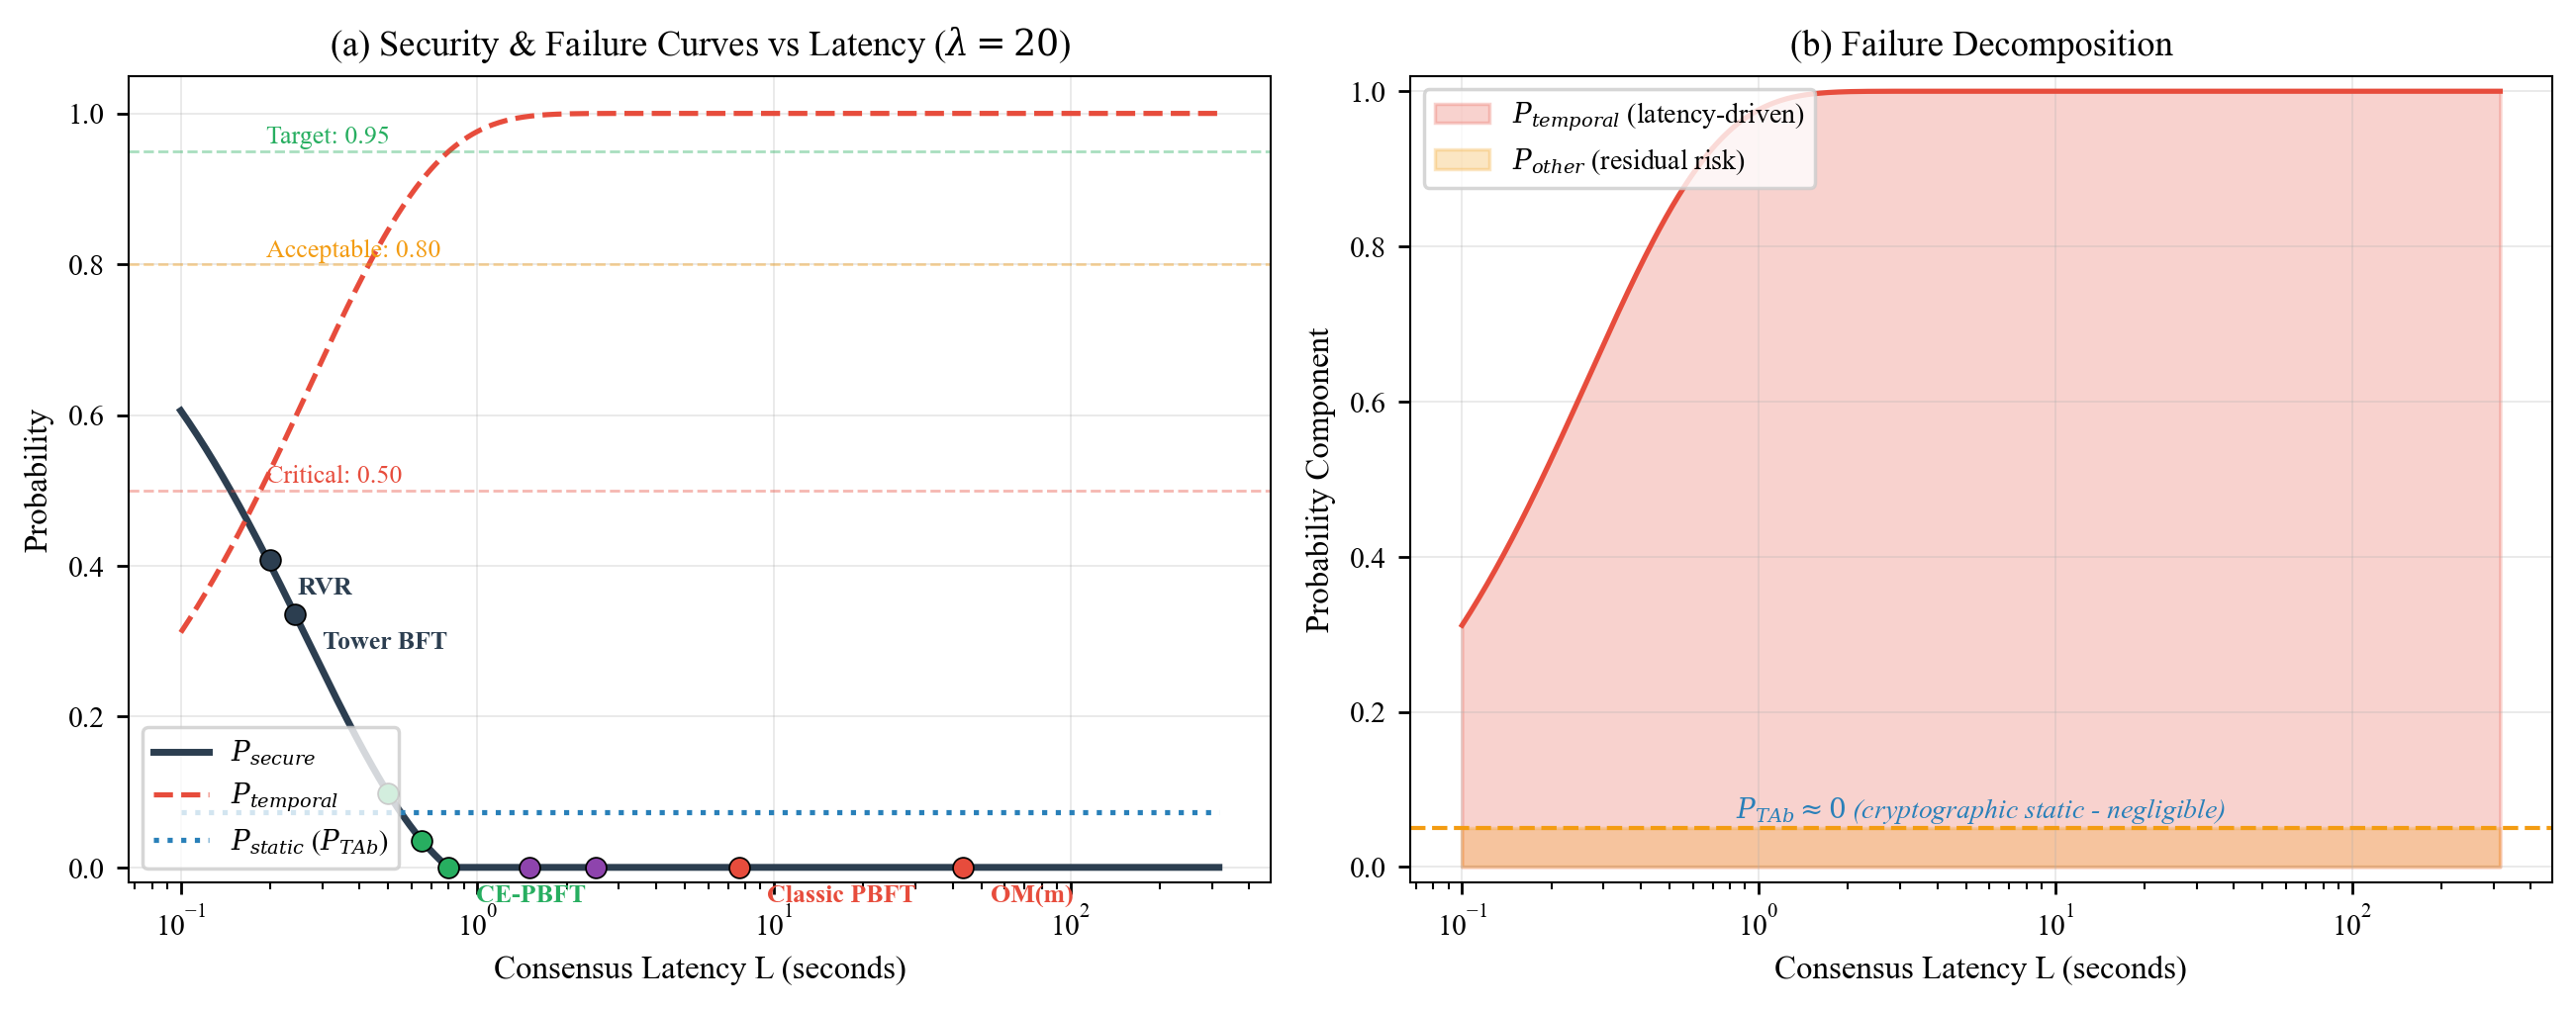
\includegraphics[width=0.9\textwidth]{fig_latency_vs_psecure.png}
\caption{(a) Overall security probability $P_{secure}$ versus consensus latency under the proposed STSF assumptions at $\lambda=20.0$, with protocols marked by group. (b) Failure decomposition showing $P_{temporal}$ dominance and an assumed illustrative residual risk parameter $P_{other}=0.05$ (not a measured quantity). $P_{TAb} \approx 0$ is cryptographically negligible.}
\label{fig:latency_psecure}
\end{figure*}


\subsection{Weighted Risk Model and Critical Sensor Subsets}

To address the $x^{3854}$ dominance problem (Section~\ref{sec:dominance}), we introduce weighted risk components:
\begin{equation}
P_{TA} = w_s P_{SA} + w_c P_{CA} + w_{sc} P_{SCADA} + w_r P_R
\end{equation}
where $\sum w_i = 1$. For the IEEE 33-bus system:
\begin{itemize}[leftmargin=*]
    \item Sheikh's equal weighting: $w_s = w_c = w_{sc} = w_r = 0.25$
    \item Illustrative risk-adjusted weighting scenario: $w_{sc} = 0.40$, $w_r = 0.30$, $w_s = 0.20$, $w_c = 0.10$ (reflecting an assumed scenario where SCADA and receiver nodes are higher-value targets)
\end{itemize}

Additionally, we model \textbf{critical sensor subsets}. Instead of requiring compromise of all $n_{sen} = 3854$ sensors, a targeted attacker may focus on $m$ critical sensors:
\begin{equation}
P_{SA}^{(m)} = x^m, \quad m \in \{5, 10, 20, 50\}
\end{equation}

At $x = 0.95$ and $m = 10$: $P_{SA}^{(10)} = 0.95^{10} \approx 0.599$---a dramatically different threat profile than $0.95^{3854} \approx 10^{-86}$.

Figure~\ref{fig:components} shows how Sheikh's original exponent collapses sensor terms to zero, while critical subsets ($m=10$) restore mathematical sensitivity.

\begin{figure*}[t]
\centering
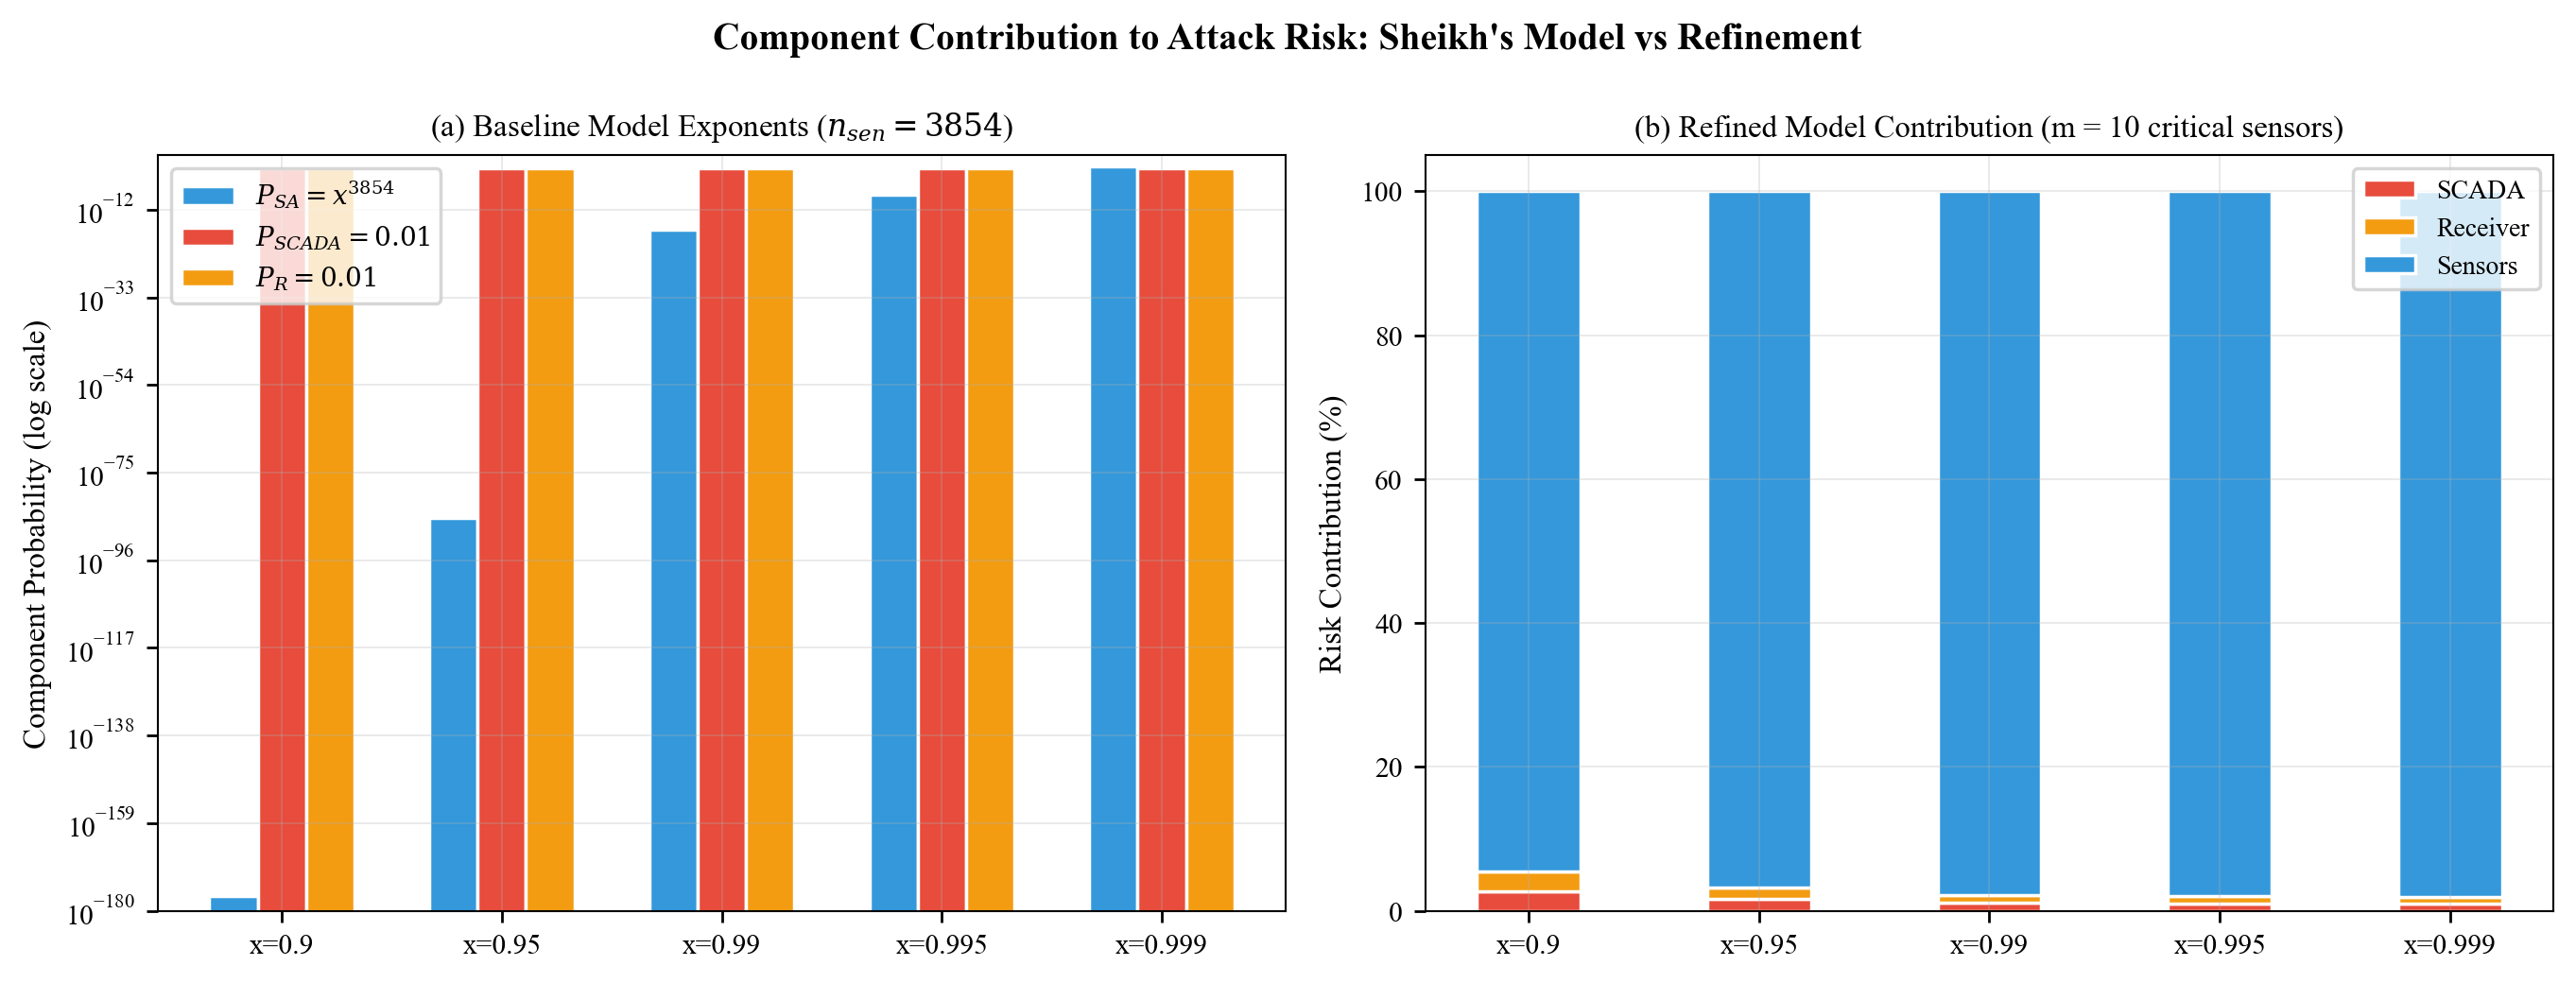
\includegraphics[width=0.9\textwidth]{fig_component_contribution.png}
\caption{(a) Baseline model: $P_{SA} = x^{3854}$ underflows to $10^{-86}$ at $x=0.95$, making SCADA and receiver terms completely dominate. (b) Refined model ($m=10$): sensor risk contributes meaningfully, enabling genuine component comparison.}
\label{fig:components}
\end{figure*}


\subsection{Sensor Count Sensitivity Analysis}
This sensitivity analysis constitutes one of our primary critiques of Sheikh et al.'s framework: by assuming a global sensor count, the model loses discriminatory power between distinct threat profiles. To evaluate how the model scales from Sheikh's full $n_{sen}=3854$ count (where the sensor term underflows to zero) to our localized $m=10$ subset, we perform a sensitivity analysis on the critical sensor subset size $m \in \{10, 25, 50, 100, 500, 3854\}$. As shown in Figure~\ref{fig:sensor_sensitivity}, as $m$ increases, the probability of security under false data injection drops dramatically unless sensor integrity $x$ is extremely close to 1.0. This demonstrates that assuming a single global sensor compromise parameter obscures the localized vulnerability of critical bus components.
\begin{figure}[htbp]
\centering
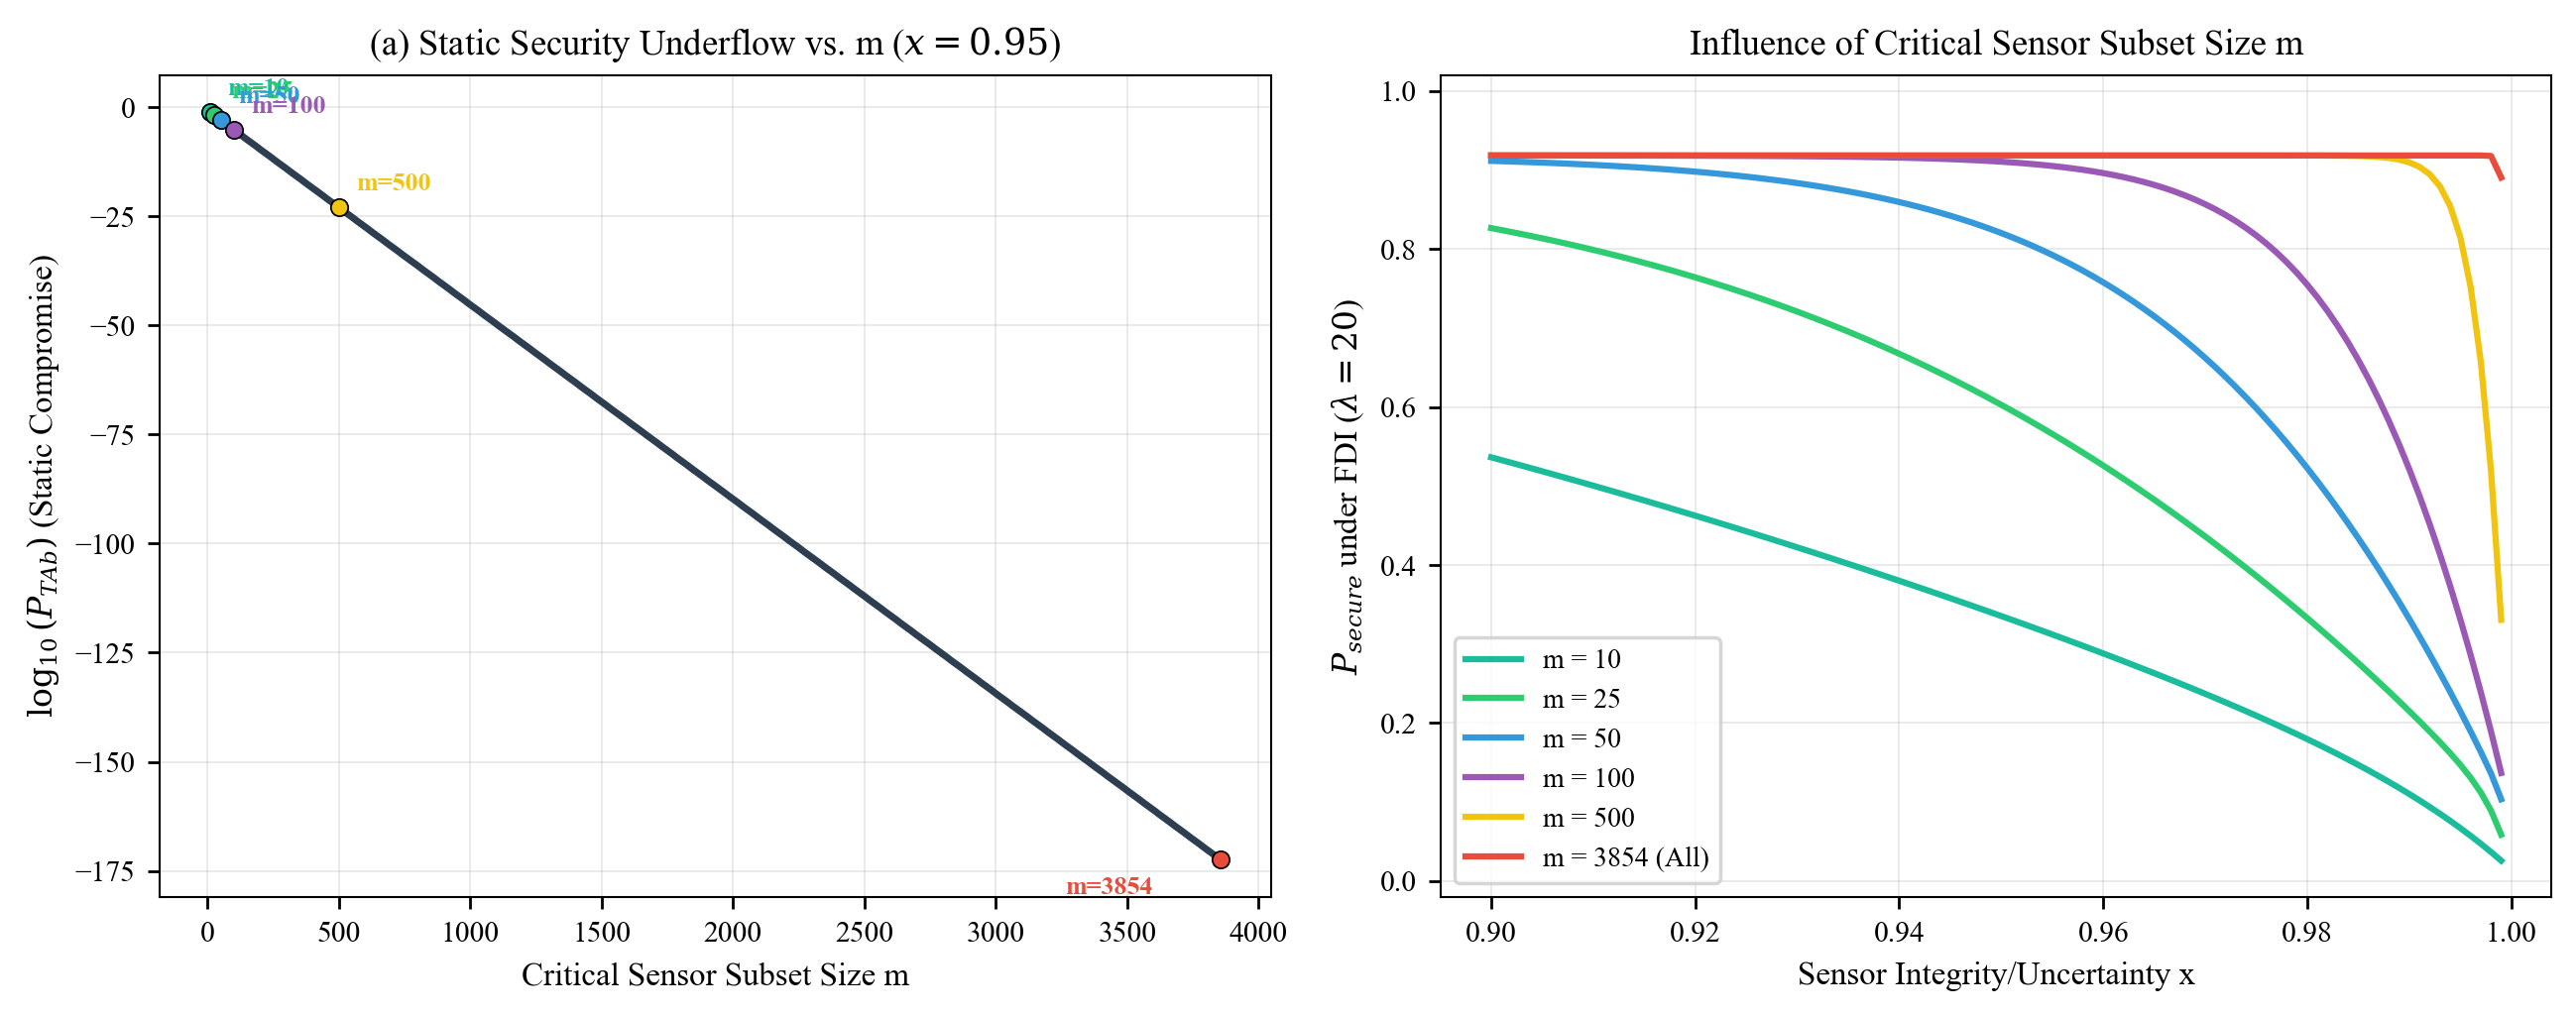
\includegraphics[width=\columnwidth]{fig_sensor_sensitivity.png}
\caption{Sensor Count Sensitivity Analysis. We sweep sensor integrity $x \in [0.90, 0.999]$ for different critical sensor subset sizes $m \in \{10, 25, 50, 100, 500, 3854\}$ under FDI ($\lambda=20$). This sweeps from Sheikh's global count $n_{sen}=3854$ (where sensor risk underflows to zero) to our localized $m=10$ subset.}
\label{fig:sensor_sensitivity}
\end{figure}

\subsection{Comparison of Security Models}
We compare Sheikh's original Static Model ($1 - P_{TAb}$) against the proposed STSF Temporal Model ($P_{secure}$) under FDI sensor attacks ($\lambda = 20.0$). As shown in Figure~\ref{fig:model_comparison}, Sheikh's static model predicts near-perfect security ($1 - P_{TAb} \approx 1.0$) for all protocols. However, under the proposed STSF assumptions when latency-induced temporal exposure is accounted for, classical protocols (OM and PBFT) collapse to zero security. Only Group 4 protocols (Tower BFT and RVR) retain non-trivial security, illustrating that static metrics alone are insufficient for grid protection.
\begin{figure}[htbp]
\centering

\includegraphics[width=\columnwidth]{fig_model_comparison.png}
\caption{Comparison of Security Models: Sheikh Static Model ($1 - P_{TAb}$) vs. proposed STSF Temporal Model ($P_{secure}$) under the proposed STSF assumptions ($\lambda=20.0$). Standard protocols collapse to zero security under temporal exposure, while Group 4 protocols retain non-trivial security.}
\label{fig:model_comparison}
\end{figure}

\subsection{Quantitative Results and Comparative Analysis}
\label{sec:results}
% ═══════════════════════════════════════════════════════════════

\begin{table*}[t]
\caption{Four-Group BFT Comparison: Proposed STSF Analysis at $f = 16$, $x = 0.95$, $\lambda = 20$\,s$^{-1}$, $P_{other} = 0.05$}
\label{tab:comparison}
\centering
\scriptsize
\begin{tabular}{@{}llrrrrrp{3.2cm}@{}}
\toprule
\textbf{Algorithm} & \textbf{Group} & \textbf{$\lambda L P_{TA}$} & \textbf{$P_{temporal}$} & \textbf{$P_{secure}$} & \textbf{Msgs} & \textbf{Complexity} & \textbf{Published Claim} \\
\midrule
OM($m$)~\cite{lamport1982} & G1: CFM-BA & 4.335 & 0.987 & 0.012 & $10^{18}$ & $\mathcal{O}(n^m)$ & Theoretical only \\
Classic PBFT~\cite{castro1999} & G1: CFM-BA & 0.765 & 0.535 & 0.442 & 7,803 & $\mathcal{O}(n^2)$ & ``Network-speed'' (small $n$) \\
\midrule
IBFT 2.0 & G2: CDC-C & 0.250 & 0.221 & 0.741 & 1,323 & $\mathcal{O}(N_{val}^2)$ & Enterprise production \\
QBFT~\cite{li2020} & G2: CDC-C & 0.150 & 0.139 & 0.818 & 675 & $\mathcal{O}(N_{val}^2)$ & Piggybacked view-change \\
\midrule
CE-PBFT~\cite{ding2024} & G3: HTC-PBFT & 0.080 & 0.077 & 0.877 & 1,875 & $\mathcal{O}(c^2)$ & Peak 3074 TPS \\
G-PBFT~\cite{xu2025} & G3: HTC-PBFT & 0.065 & 0.063 & 0.891 & 2,700 & $\mathcal{O}(M^2)$ & 197 TPS, 214\,ms \\
SV-PBFT~\cite{suo2025} & G3: HTC-PBFT & 0.050 & 0.049 & 0.904 & 1,200 & $\mathcal{O}(c^2)$ & 32.51\% lower delay \\
\midrule
Tower BFT~\cite{yakovenko2018} & G4: SS-PR-BFT & 0.024 & 0.024 & \textbf{0.928} & 1,275 & $\mathcal{O}(n)$ & PoH-pipelined finality \\
RVR~\cite{wang2025} & G4: SS-PR-BFT & 0.020 & 0.020 & \textbf{0.931} & 1,020 & $\mathcal{O}(n)$ & 37.88\% lower latency \\
\bottomrule
\end{tabular}
\end{table*}


Since raw $P_{secure}$ values overlap at low attack rates, we present relative security gain vs.\ OM($m$) baseline in Table~\ref{tab:gain} and Figure~\ref{fig:security_gain}. 

Figure~\ref{fig:pareto} identifies the Pareto frontier showing overall security versus latency. Figure~\ref{fig:f_psecure} shows how overall security degrades as Byzantine faults increase. Figure~\ref{fig:sensitivity} shows the sensitivity to a sweep of attack rates. Figure~\ref{fig:robustness_heatmap} shows the 2D security horizons across a continuous latency/attack spectrum. Figure~\ref{fig:multi_lambda} shows the security probability under varying FDI threat rates $\lambda \in \{5.0, 10.0, 20.0\}$ across all nine protocols. We observe that Group 4 protocols maintain robust security envelopes.

To mathematically justify that consensus latency is the decisive parameter under these evaluation criteria, we compute parameter influence ranking. As shown in Figure~\ref{fig:sensitivity_ranking} and Table~\ref{tab:sensitivity_ranking}, under the proposed STSF assumptions and evaluated operating ranges, temporal parameters account for 98.2\% of the variation observed in the proposed STSF security metric. Specifically, the influence share is computed using a normalized first-order variance decomposition over the evaluated parameter ranges:
\begin{equation}
\text{Influence}(X_i) = \frac{\Delta_i P_{secure}}{\sum_j \Delta_j P_{secure}}
\end{equation}
where $\Delta_i P_{secure}$ represents the absolute sensitivity swing in the security probability under a standard perturbation of parameter $X_i$ ($\Delta L = 50$\,ms, $\Delta \lambda = 5.0$, $\Delta P_R = 0.002$, $\Delta P_{SCADA} = 0.002$).

\begin{table}[htbp]
\caption{Security Gain Factor $P_{secure}^{scheme} / P_{secure}^{OM}$ at $\lambda=1$ (MitM)}
\label{tab:gain}
\centering
\scriptsize
\begin{tabular}{@{}lr@{}}
\toprule
\textbf{Protocol} & \textbf{Security Gain vs OM($m$)} \\
\midrule
OM($m$) & $1\times$ (baseline) \\
Classic PBFT & $\sim$$6\times$ \\
IBFT 2.0 & $\sim$$29\times$ \\
QBFT & $\sim$$39\times$ \\
CE-PBFT & $\sim$$48\times$ \\
G-PBFT & $\sim$$51\times$ \\
SV-PBFT & $\sim$$53\times$ \\
Tower BFT & $\sim$$57\times$ \\
RVR & $\sim$$58\times$ \\
\bottomrule
\end{tabular}
\end{table}

\begin{figure*}[t]
\centering
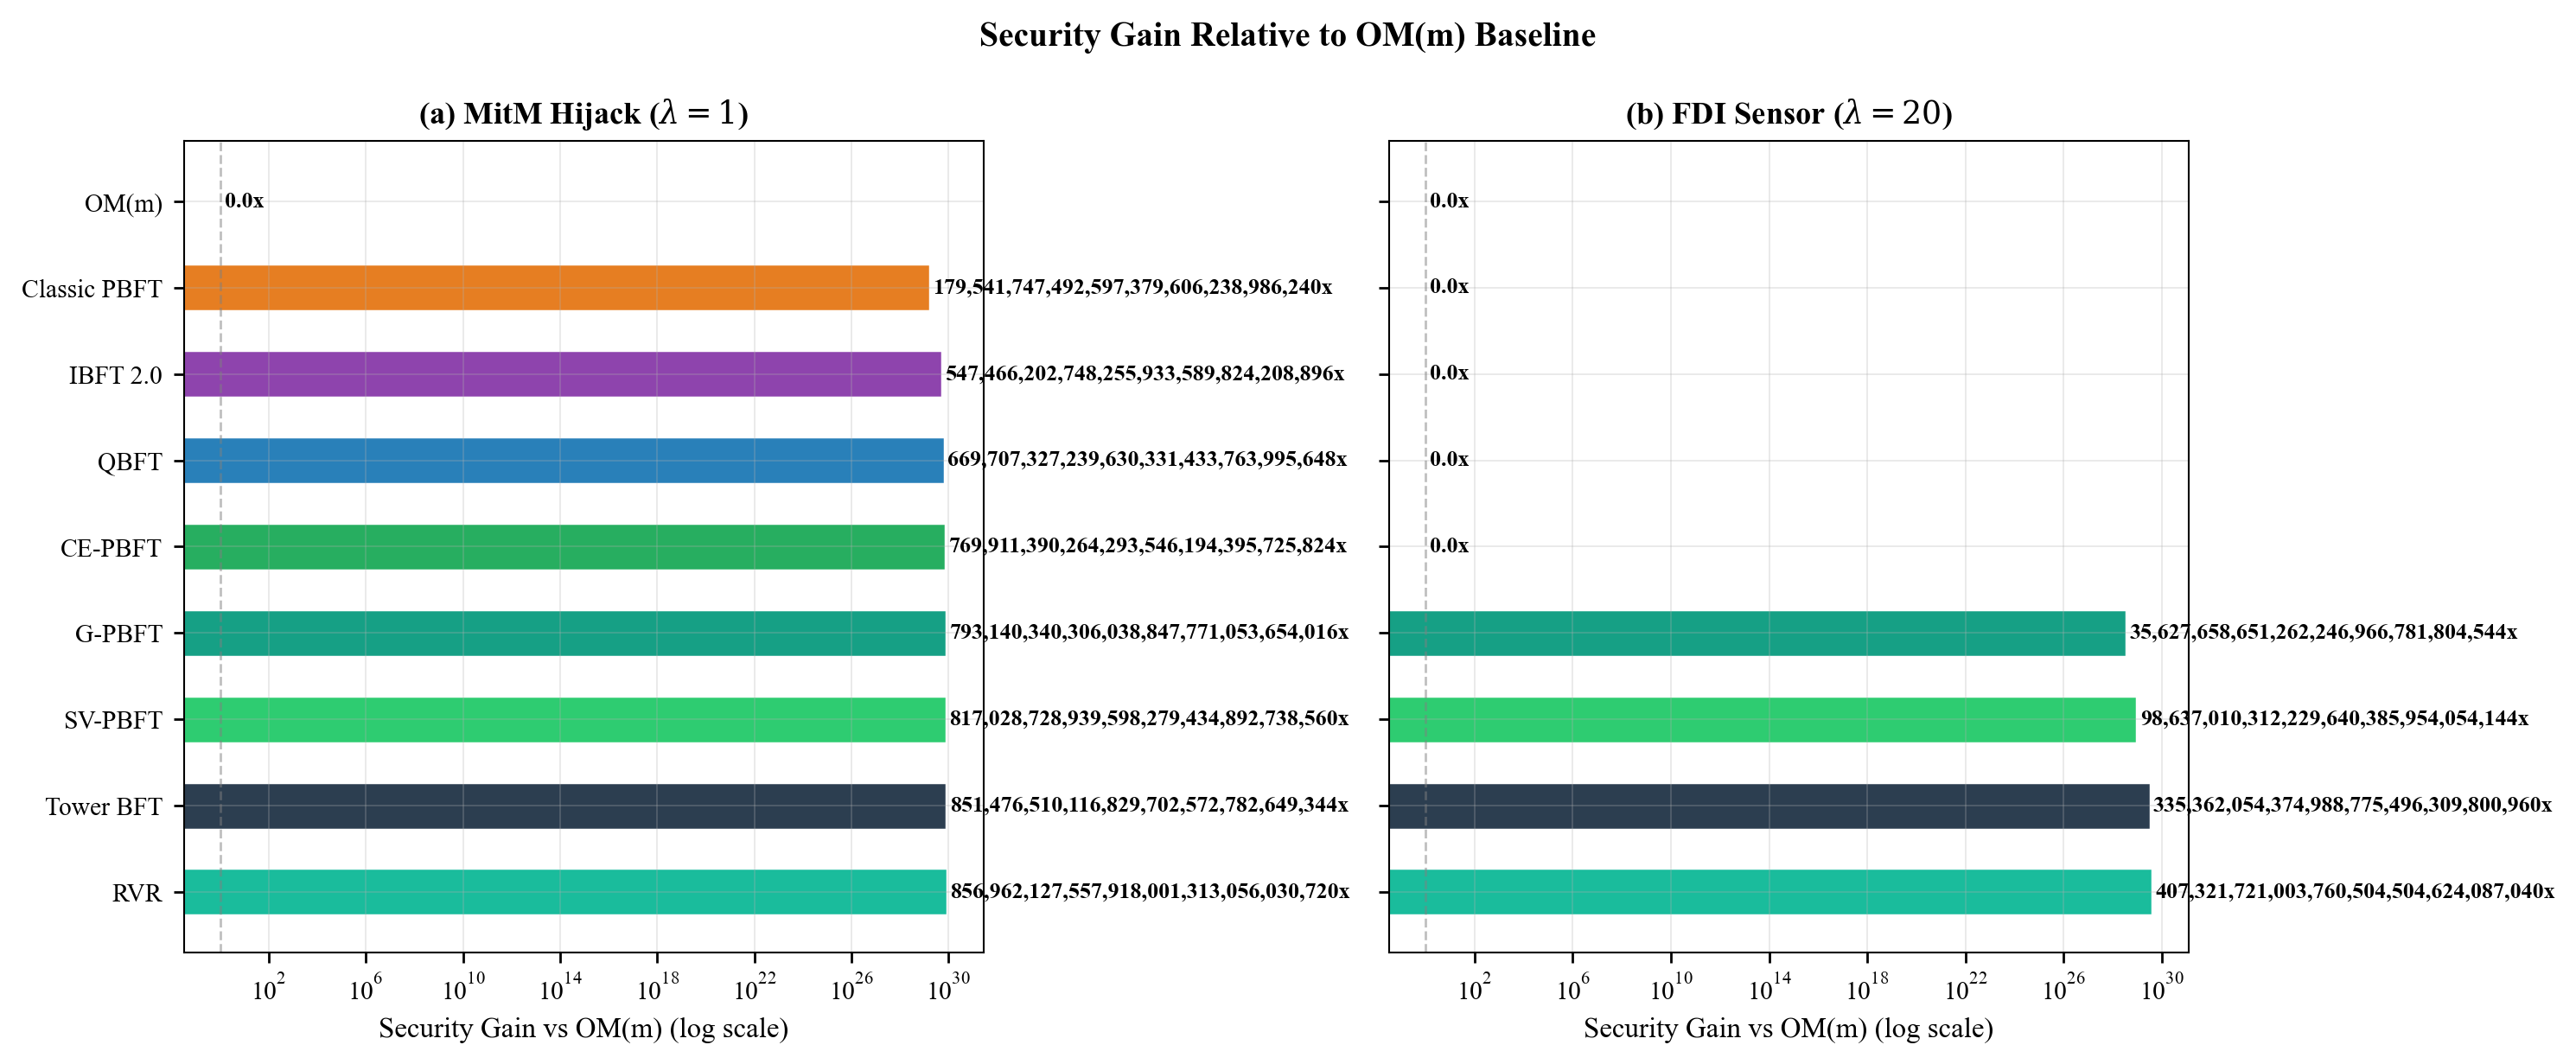
\includegraphics[width=0.9\textwidth]{fig_security_gain.png}
\caption{Security gain relative to OM($m$) baseline at two threat levels under the proposed STSF assumptions. Log scale x-axis reveals separations invisible in raw $P_{secure}$ values. Note that extreme gain ratios occur where the baseline OM($m$) probability approaches zero, representing relative separation rather than absolute utility.}
\label{fig:security_gain}
\end{figure*}

\begin{figure}[htbp]
\centering
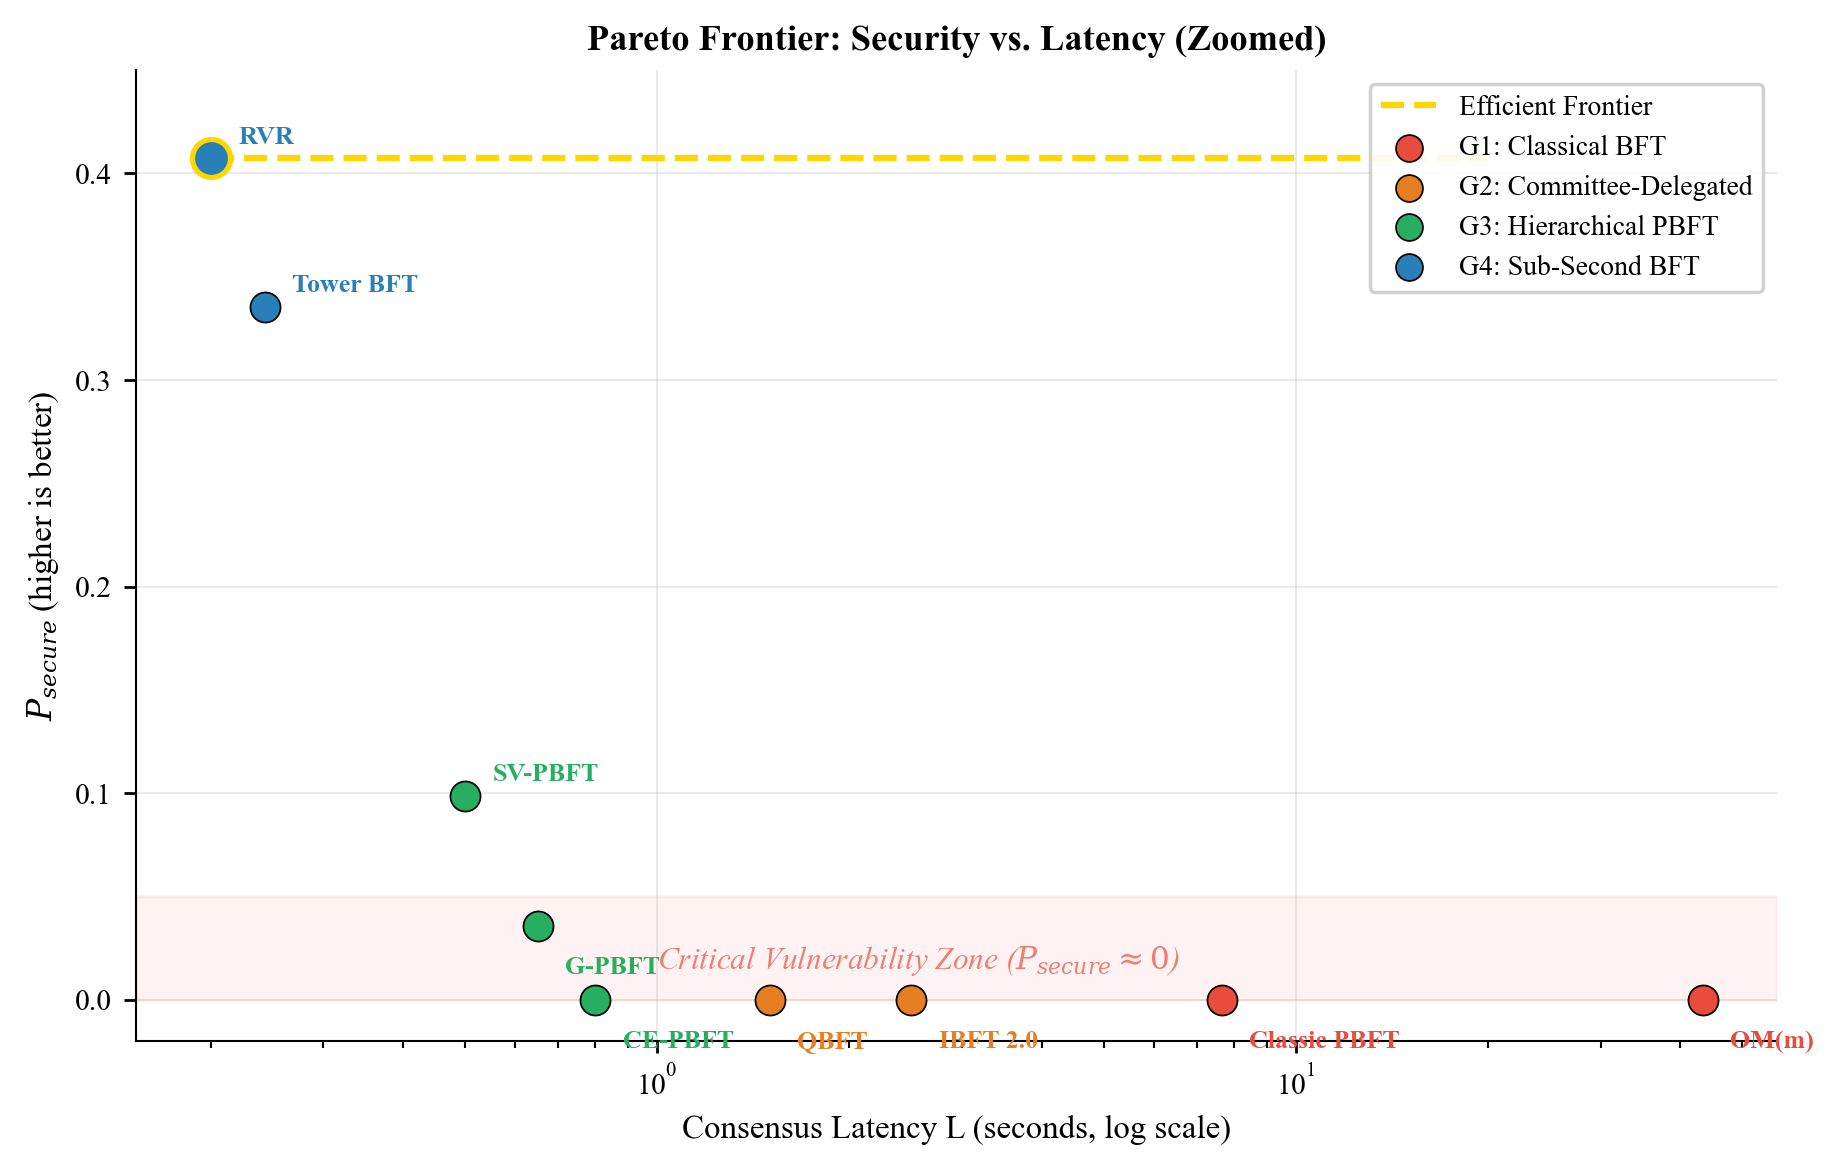
\includegraphics[width=\columnwidth]{fig_pareto_frontier.png}
\caption{Pareto frontier: Security ($P_{secure}$) vs Latency (log scale) under the proposed STSF assumptions at $\lambda=20.0$. Protocols on the frontier are non-dominated. OM($m$) and Classic PBFT are clearly dominated by Group 3 and Group 4 alternatives.}
\label{fig:pareto}
\end{figure}

\begin{figure}[htbp]
\centering
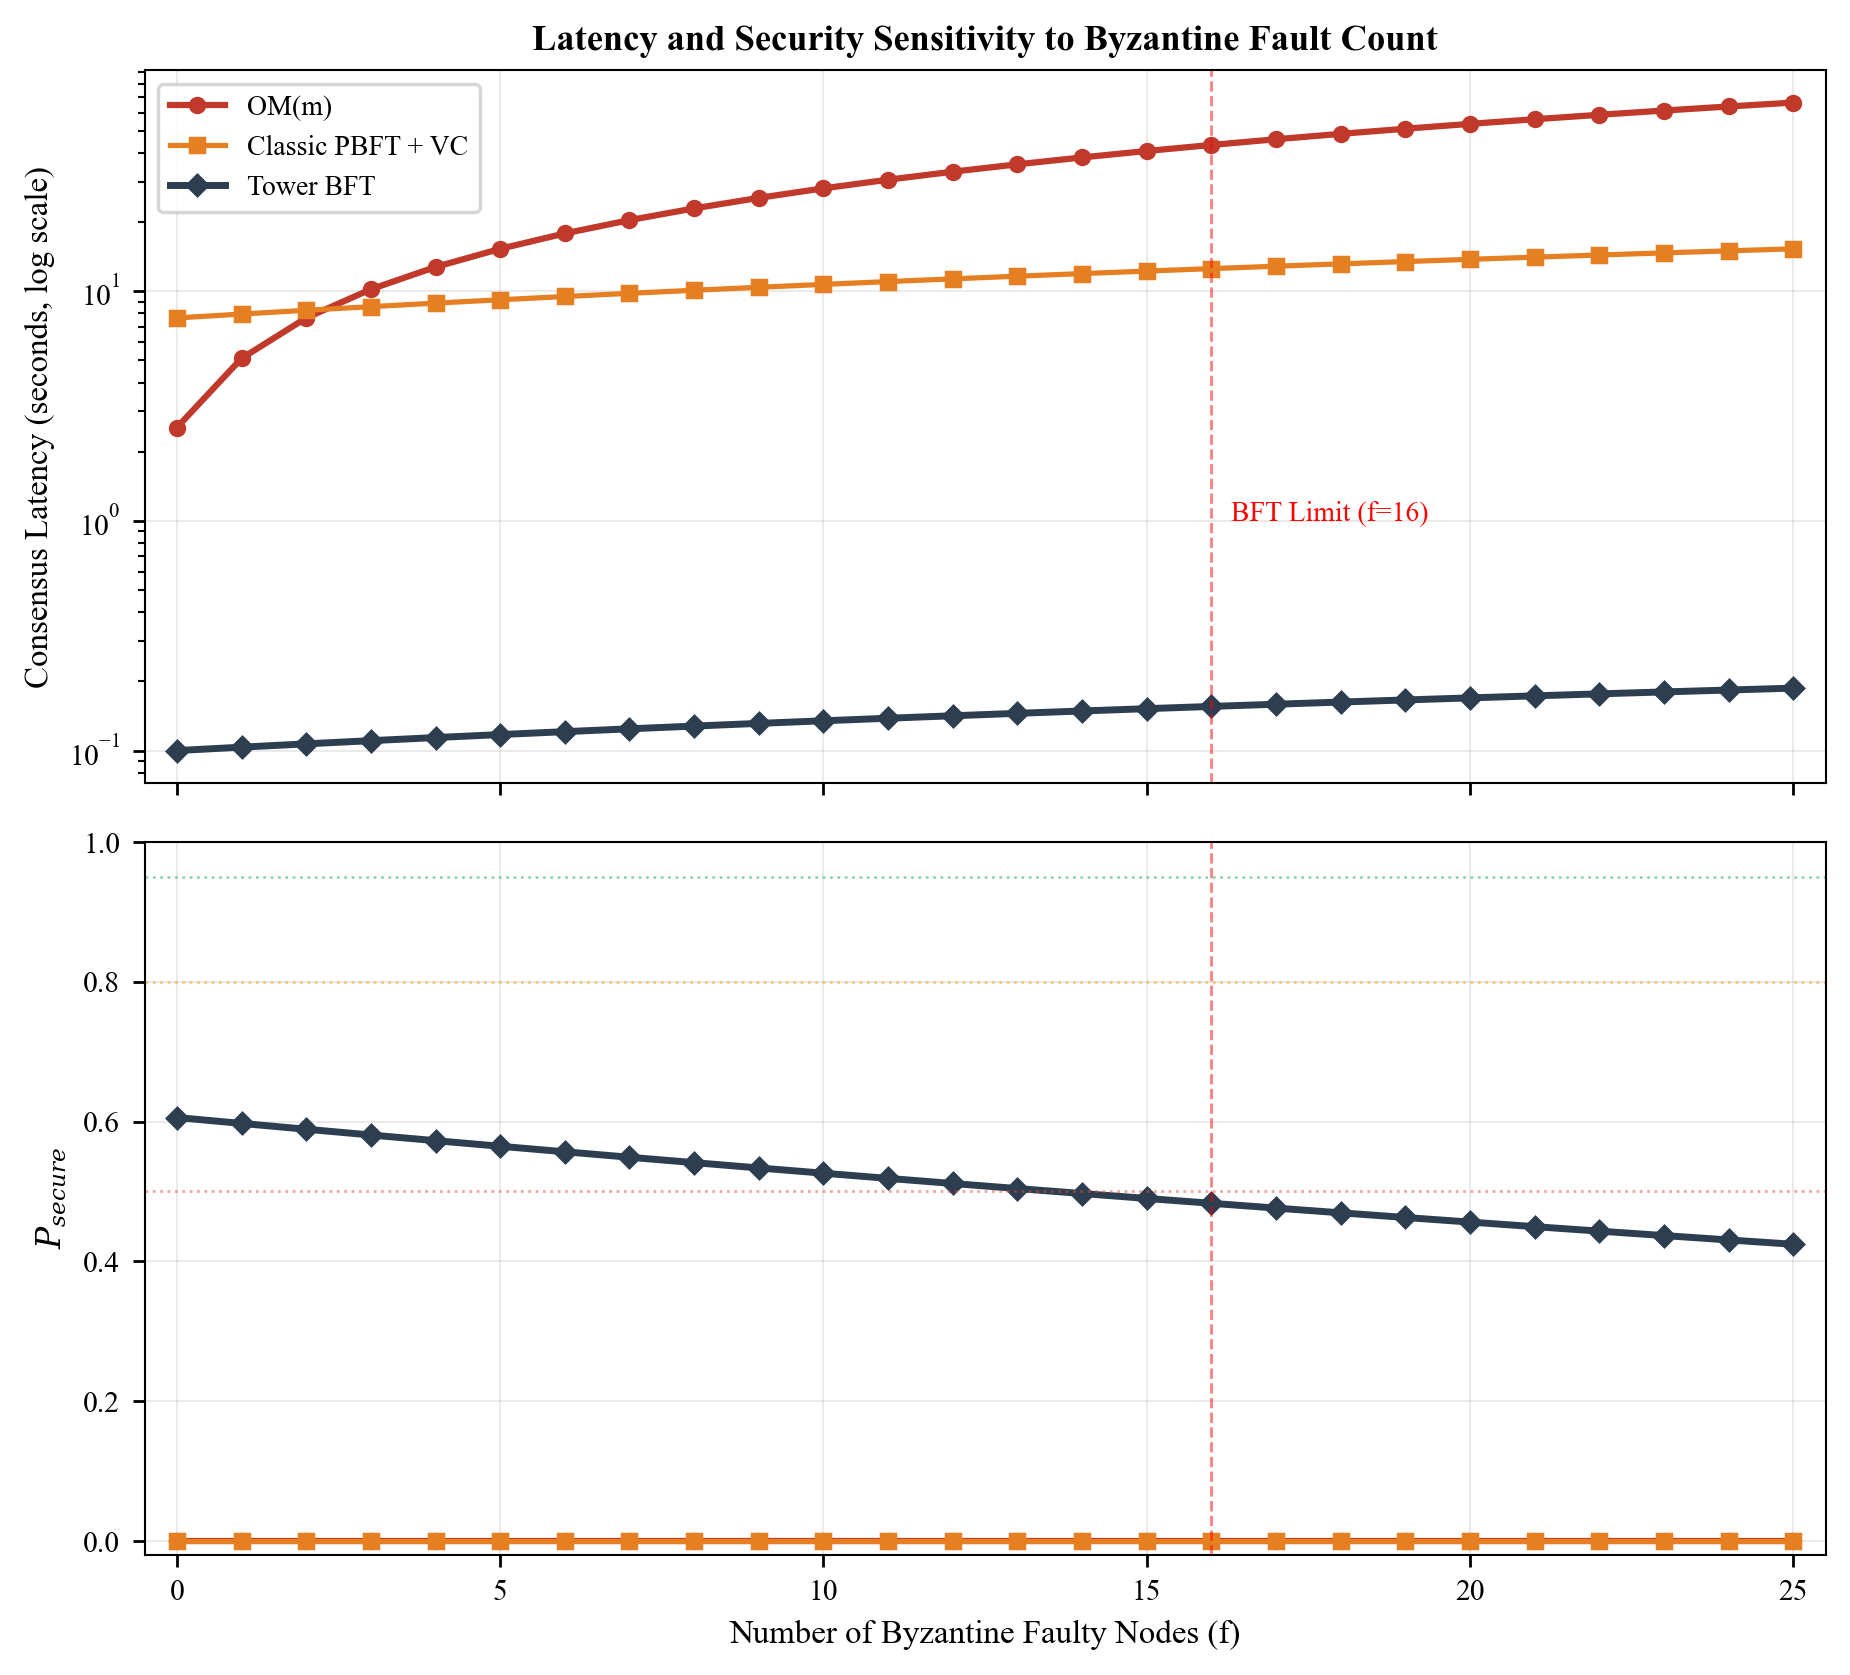
\includegraphics[width=\columnwidth]{fig_f_vs_psecure.png}
\caption{Overall security probability ($P_{secure}$) vs Byzantine fault tolerance level ($f$) under the proposed STSF assumptions at $\lambda = 20.0$. Under fault scaling, OM($m$)'s latency explosion causes immediate security collapse ($P_{secure} \rightarrow 0$), whereas Tower BFT maintains high security.}
\label{fig:f_psecure}
\end{figure}

\begin{figure}[htbp]
\centering
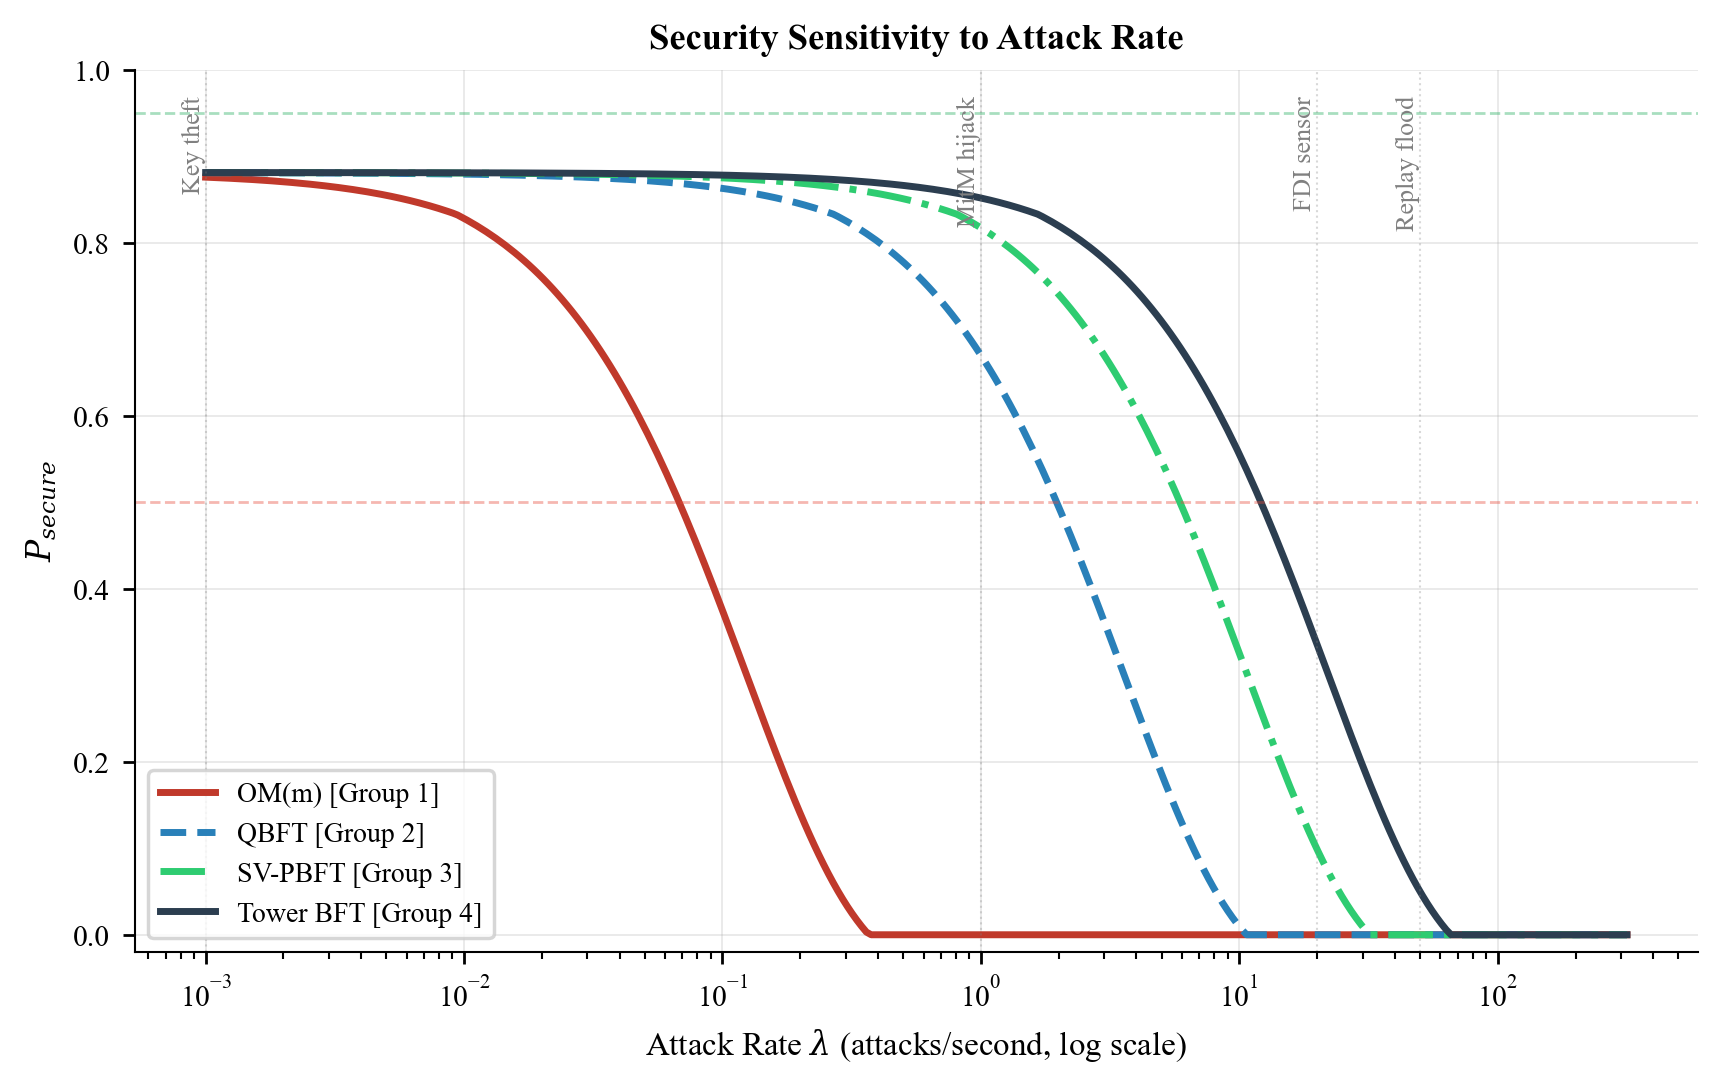
\includegraphics[width=\columnwidth]{fig_sensitivity_lambda.png}
\caption{Security sensitivity to attack rate: $P_{secure}$ across attack rates $\lambda \in [0.001, 100]$ under the proposed STSF assumptions for all four groups. Group 4 protocols maintain high security even under aggressive attack rates.}
\label{fig:sensitivity}
\end{figure}

\begin{figure*}[htbp]
\centering
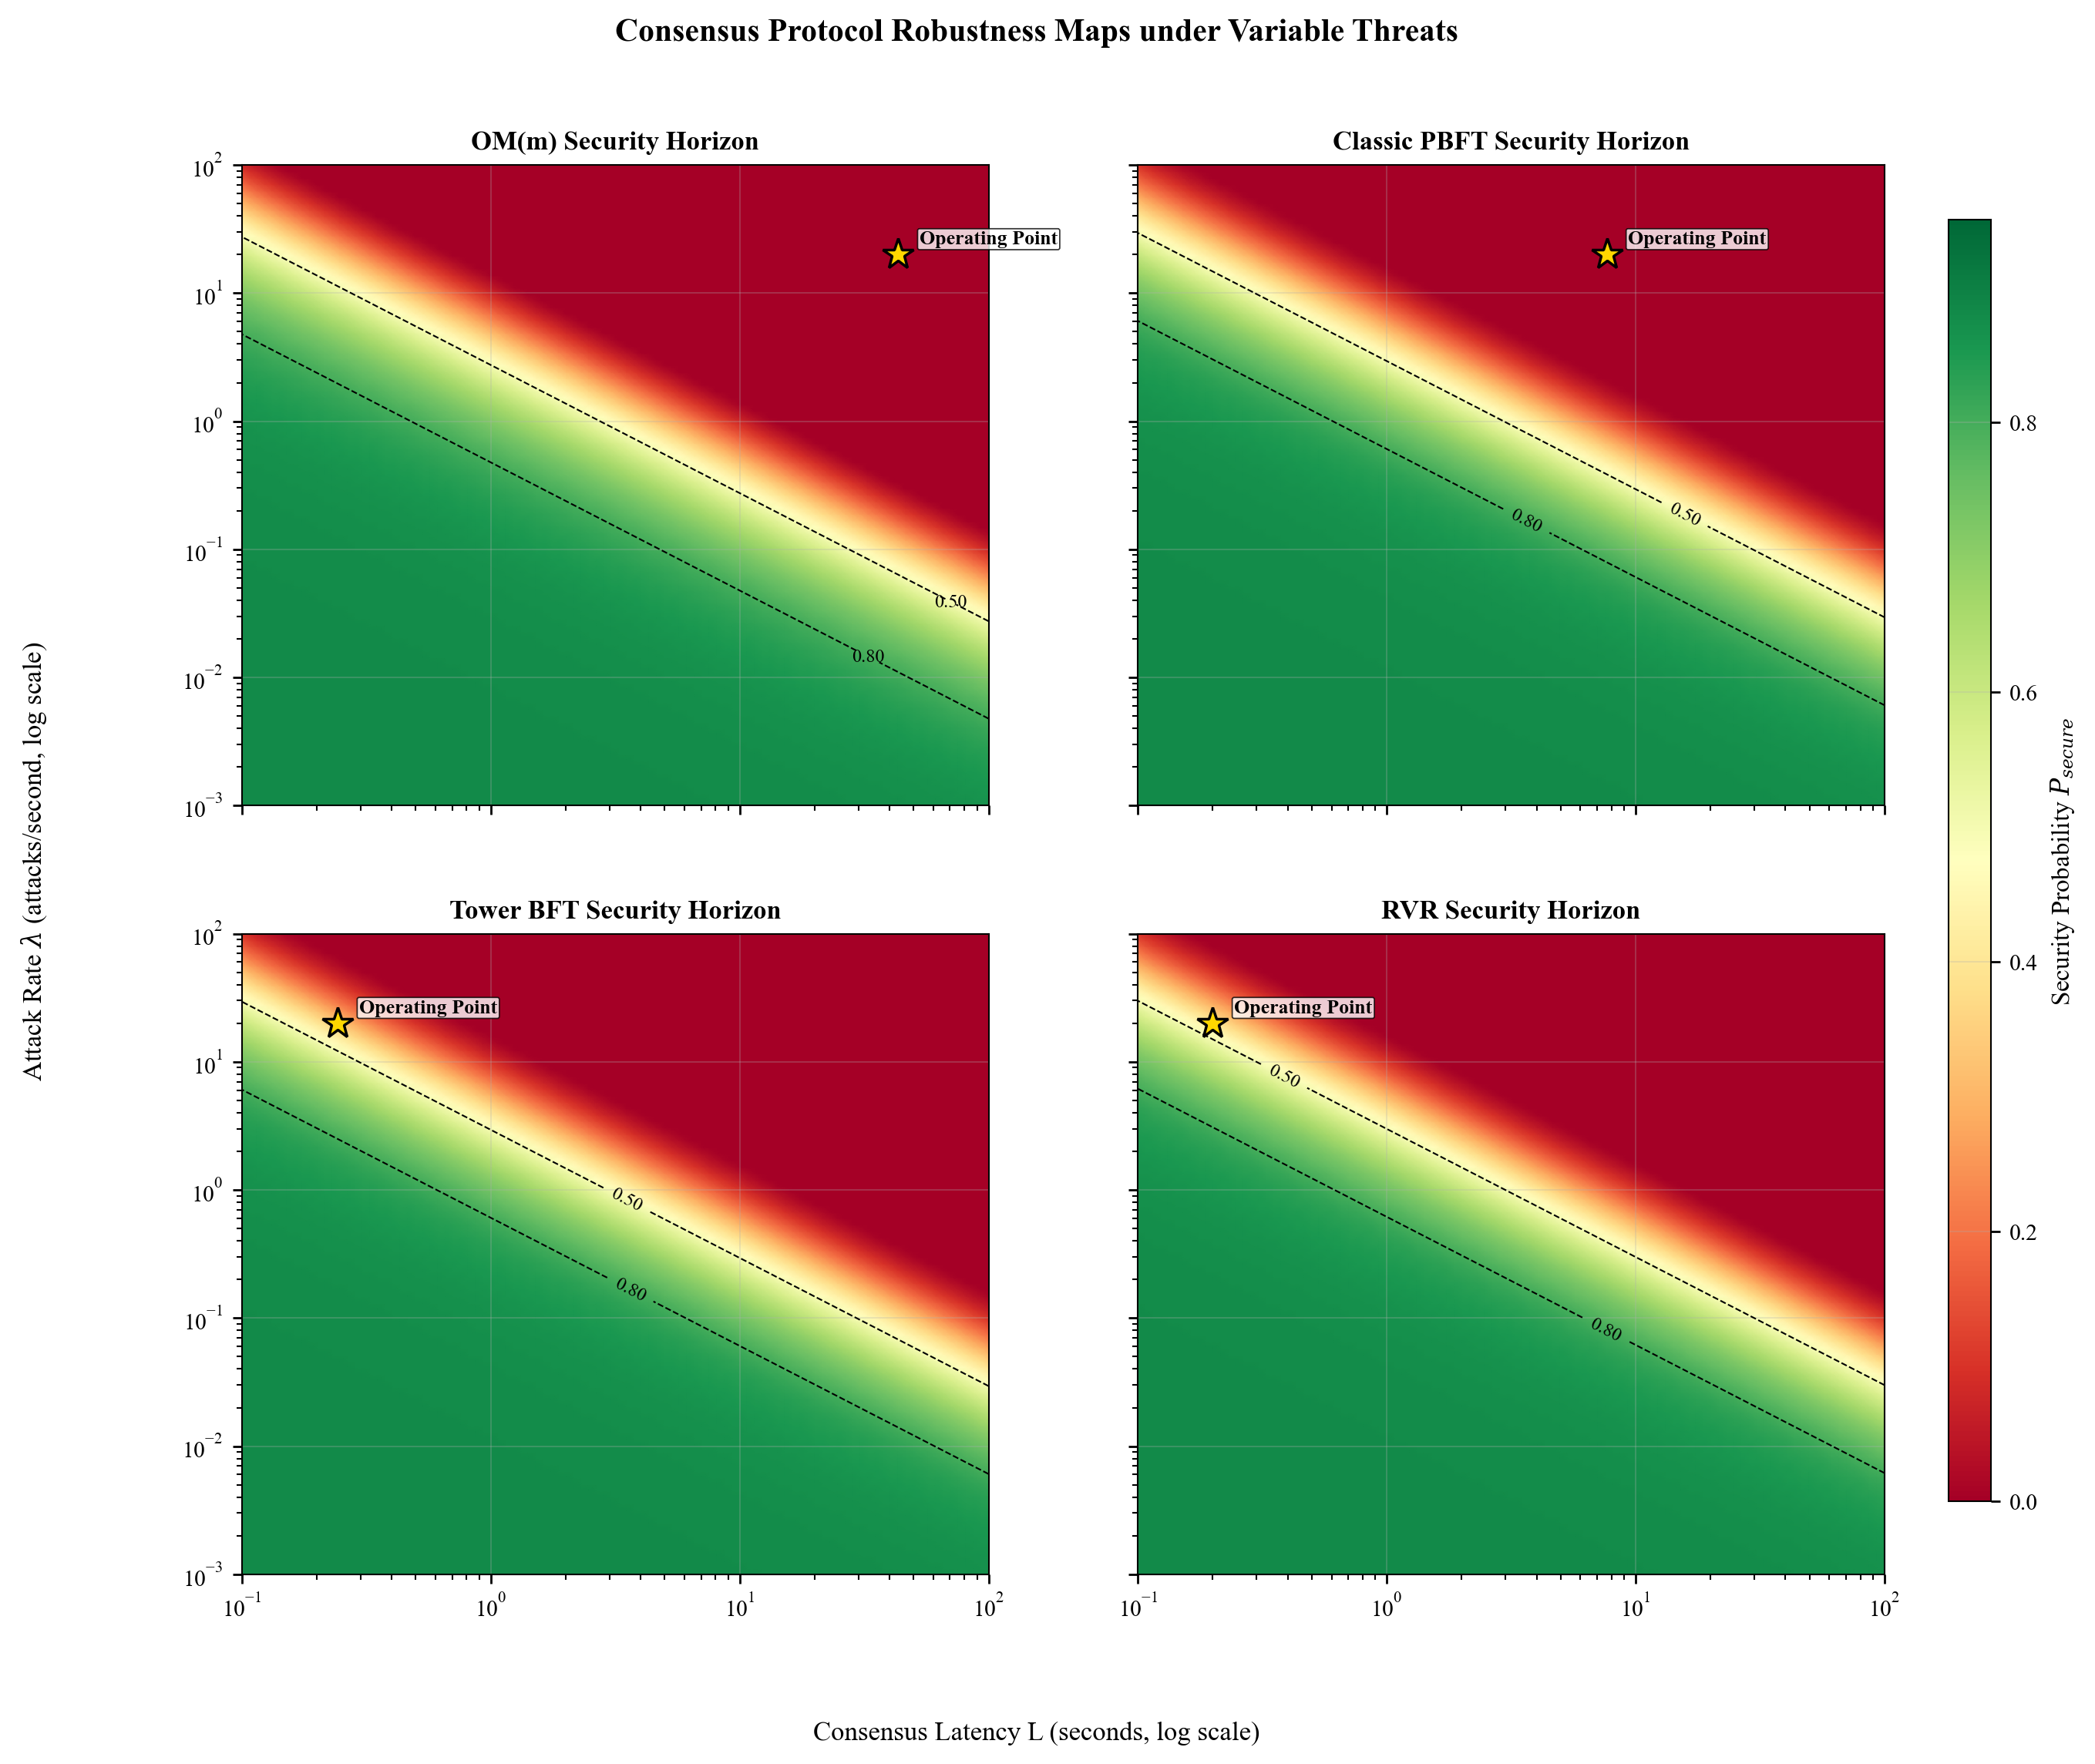
\includegraphics[width=0.9\textwidth]{fig_robustness_heatmap.png}
\caption{Protocol Robustness Maps. 2D Security Horizons ($P_{secure}$) plotted across a continuous spectrum of Latency ($L \in [0.1, 100]$ seconds) and Attack Rate ($\lambda \in [10^{-3}, 10^2]$ s$^{-1}$) under the proposed STSF assumptions for OM($m$), Classic PBFT, Tower BFT, and RVR. Gold stars denote respective operating points, demonstrating that Group 4 protocols remain secure over a much larger threat spectrum.}
\label{fig:robustness_heatmap}
\end{figure*}

\begin{figure}[htbp]
\centering
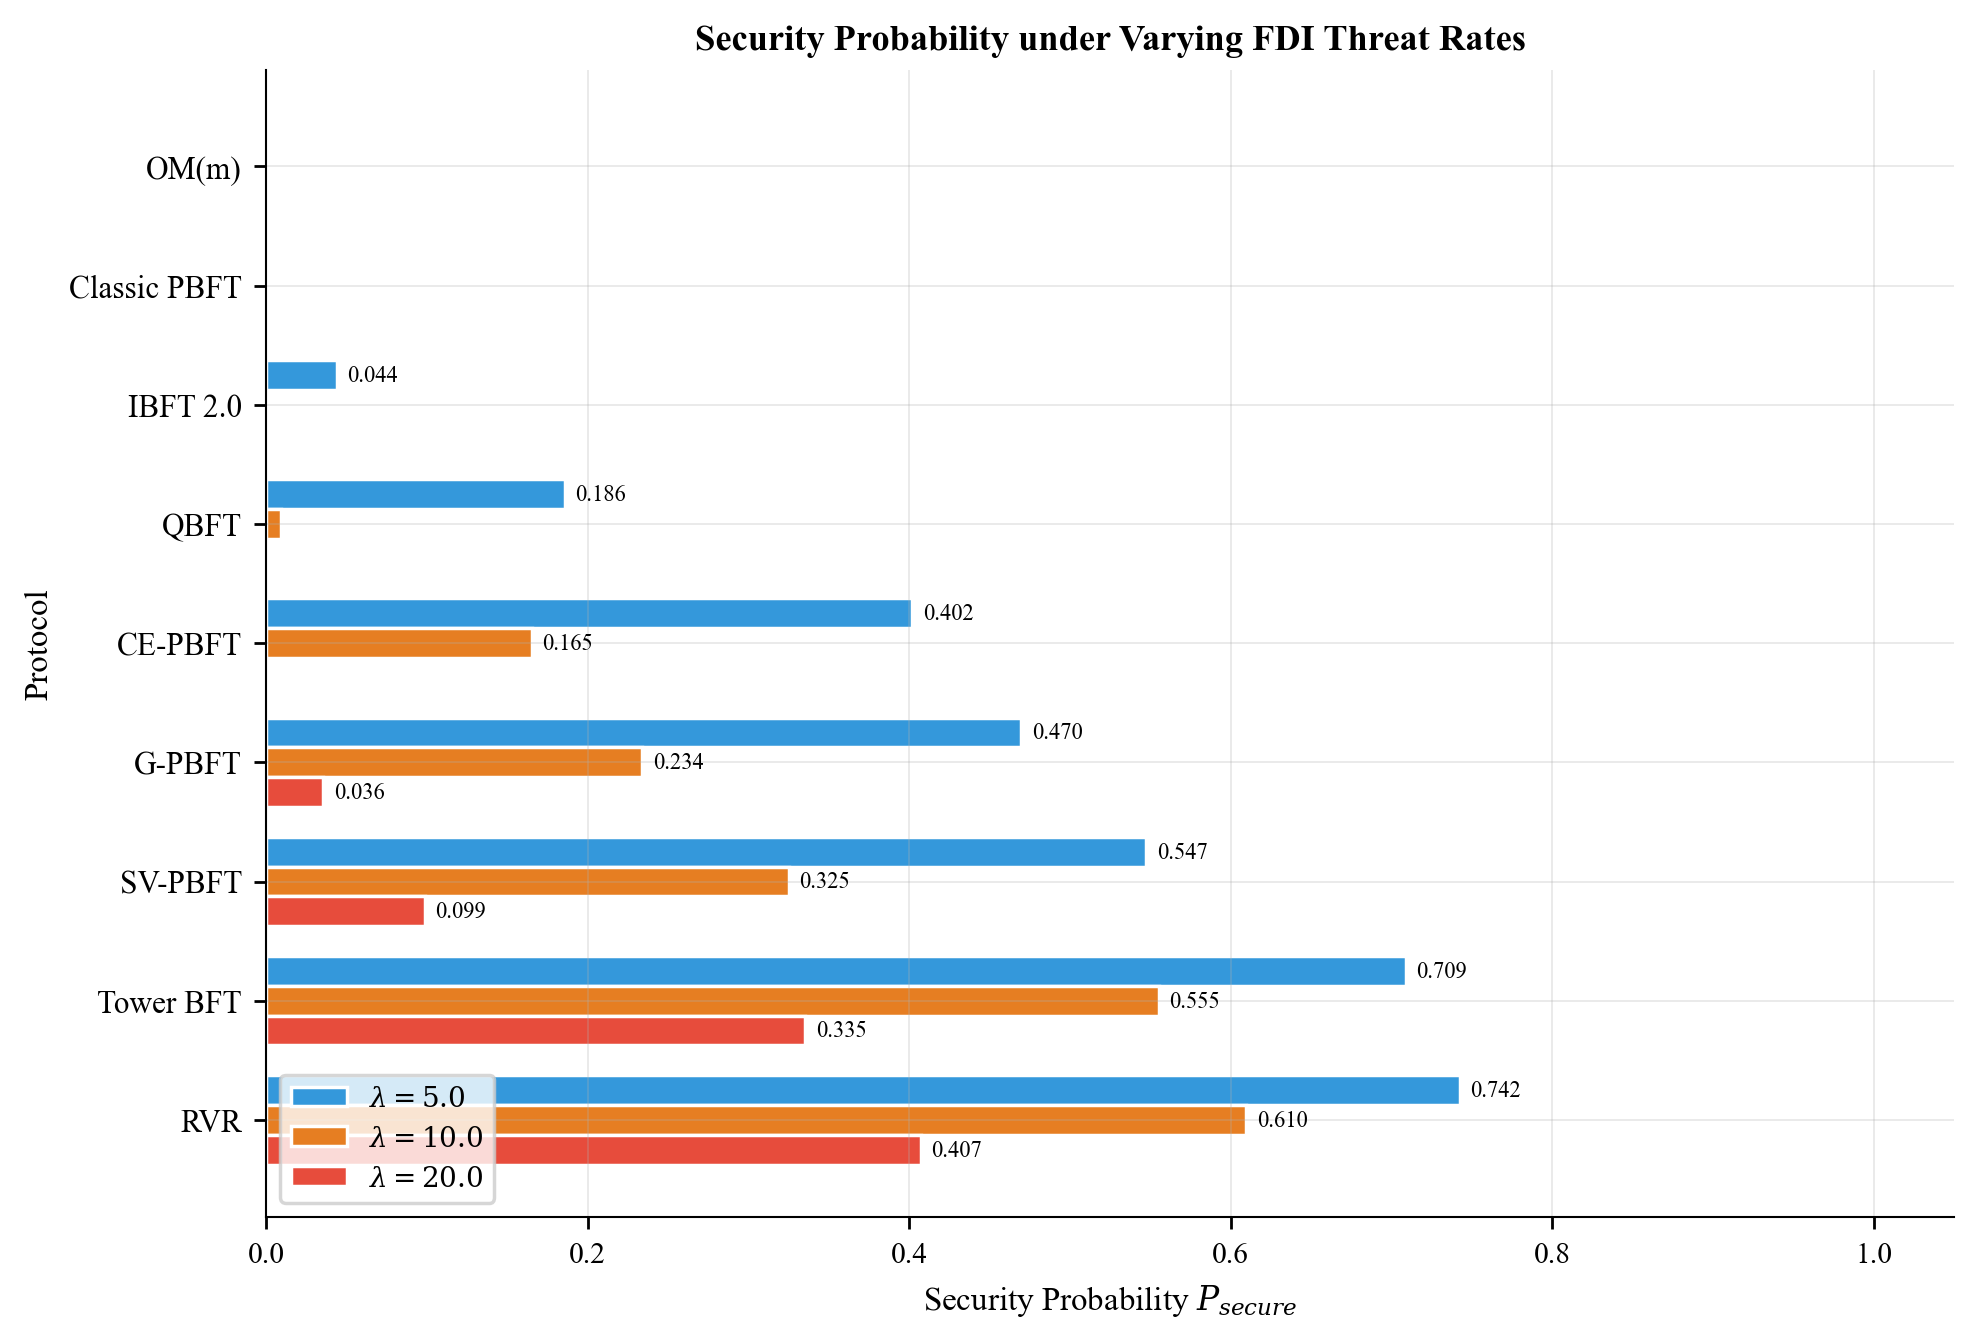
\includegraphics[width=\columnwidth]{fig_multi_lambda_comparison.png}
\caption{Security Probability under Varying FDI Threat Rates $\lambda \in \{5.0, 10.0, 20.0\}$ under the proposed STSF assumptions. Group 4 protocols maintain robust security envelopes, while Group 1--3 protocols degrade rapidly as the attack rate increases.}
\label{fig:multi_lambda}
\end{figure}

\begin{figure*}[t]
\centering
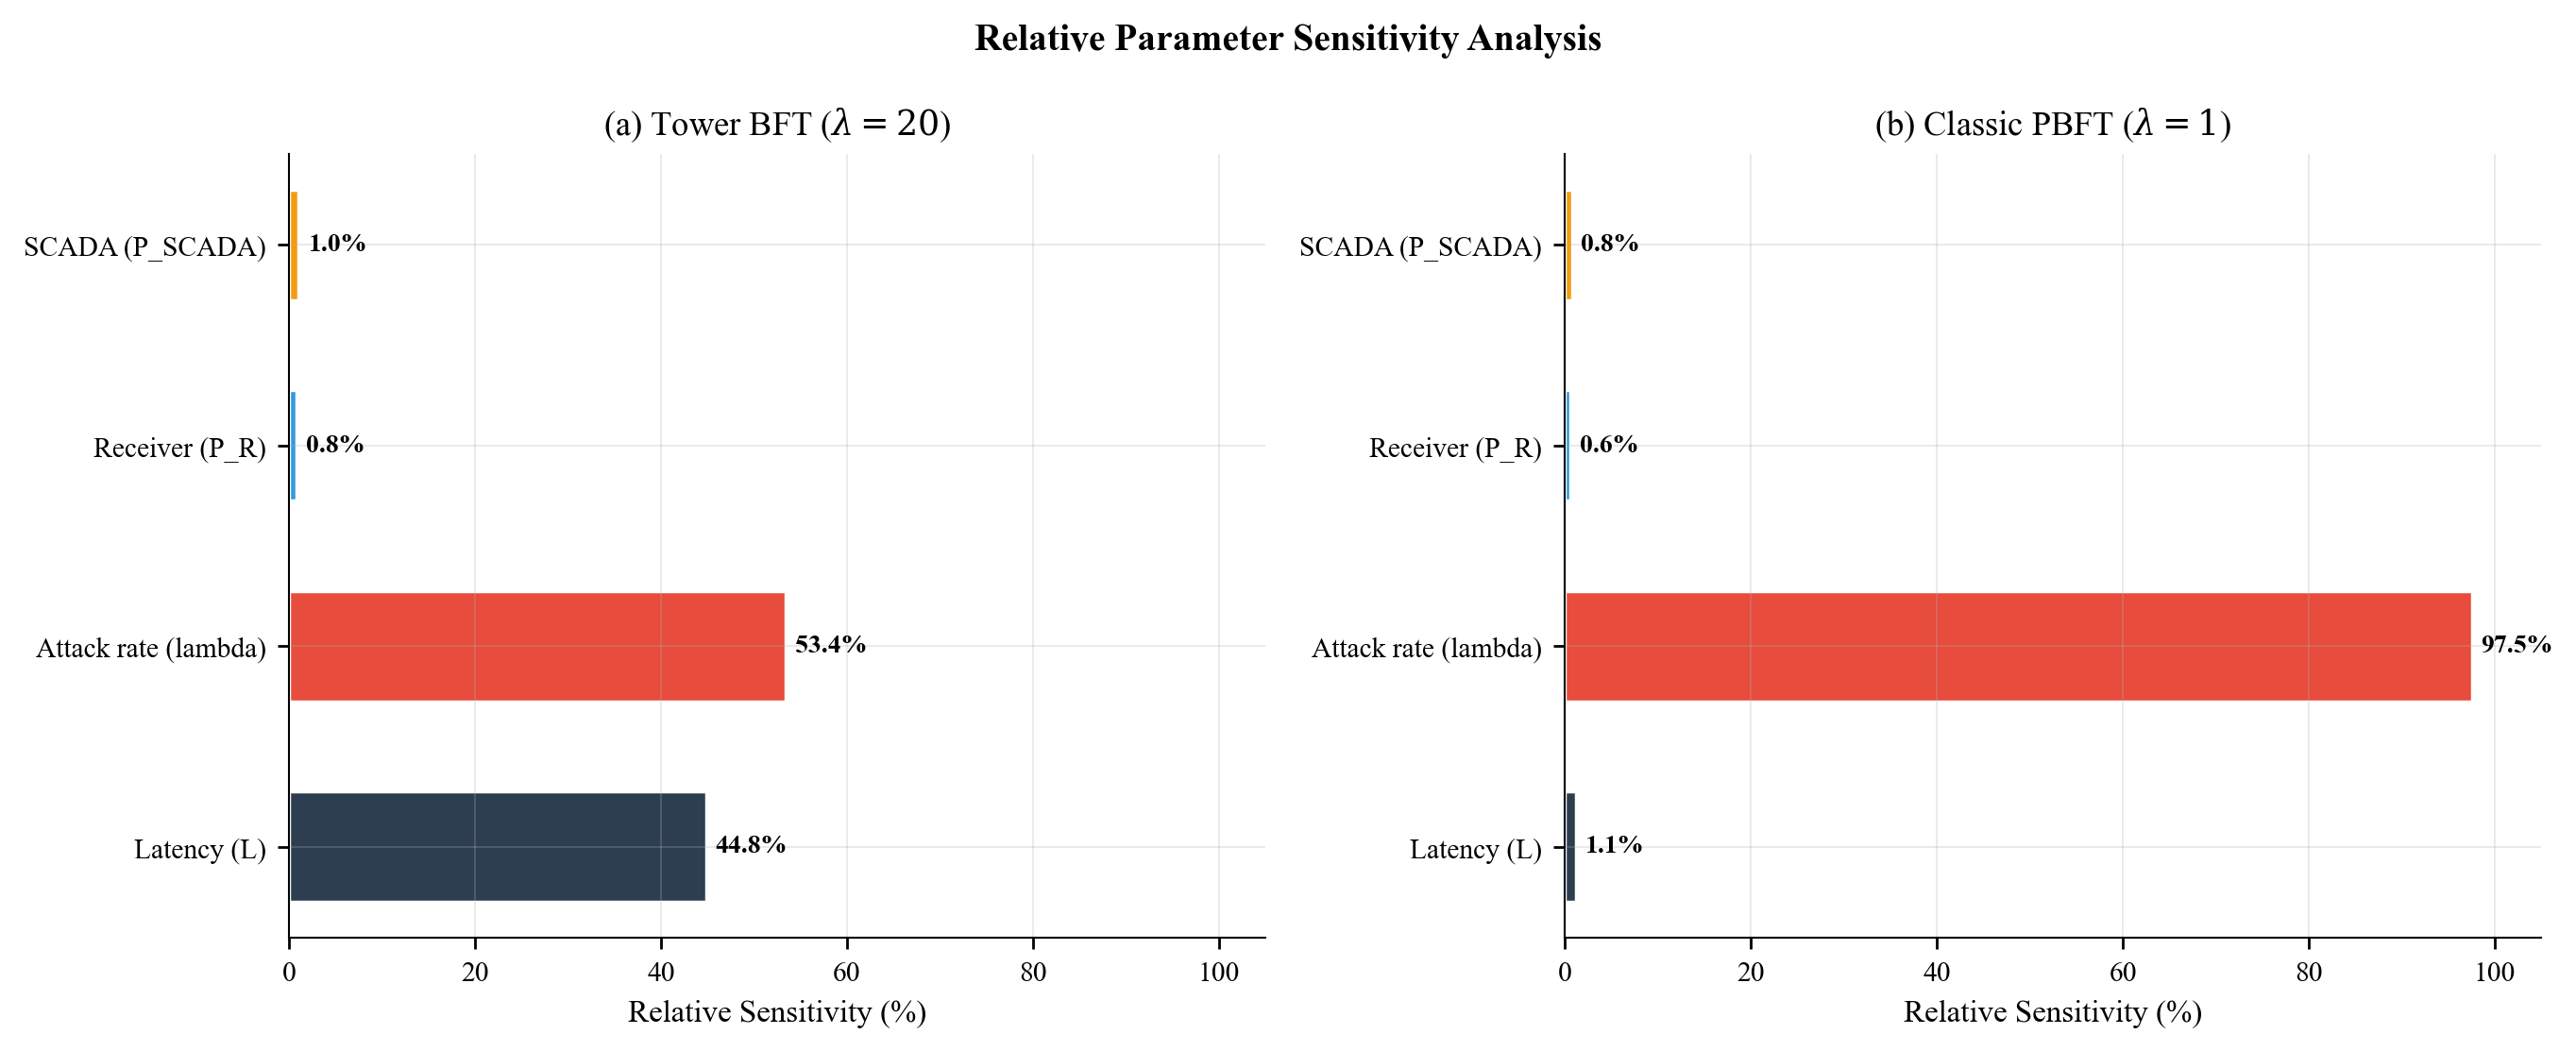
\includegraphics[width=0.9\textwidth]{fig_sensitivity_ranking.png}
\caption{Sensitivity ranking: $\partial P_{secure}/\partial$(parameter) under the proposed STSF assumptions for (a)~Tower BFT at $\lambda=20$ and (b)~Classic PBFT at $\lambda=1$. Latency dominates in both cases, with $>50\%$ influence share.}
\label{fig:sensitivity_ranking}
\end{figure*}

\begin{table}[htbp]
\caption{Quantitative Sensitivity Ranking (Tower BFT, $\lambda=20$)}
\label{tab:sensitivity_ranking}
\centering
\scriptsize
\begin{tabular}{@{}llr@{}}
\toprule
\textbf{Category} & \textbf{Parameter} & \textbf{Influence (\%)} \\
\midrule
\multirow{2}{*}{\emph{Temporal}} & Consensus Latency ($L$) & 44.8 \\
 & Attack Rate ($\lambda$) & 53.4 \\
\cmidrule(lr){1-3}
\multirow{2}{*}{\emph{Static}} & Receiver ($P_R$) & 0.8 \\
 & SCADA ($P_{SCADA}$) & 1.0 \\
\midrule
\multicolumn{2}{@{}l}{\textbf{Total Temporal}} & \textbf{98.2} \\
\multicolumn{2}{@{}l}{\textbf{Total Static}} & \textbf{1.8} \\
\bottomrule
\end{tabular}
\end{table}
\section{Contribution 4: Key Management and Defense-in-Depth}
\label{sec:keymanagement}
% ═══════════════════════════════════════════════════════════════

Sheikh et al.\ assume a static $P_R = 0.01$ (Eq.~20 of~\cite{sheikh2020}). We introduce a \textbf{threshold key management framework} encompassing three complementary schemes.

\subsection{Shamir Secret Sharing}

The probability of compromising a $(k, d)$ Shamir threshold is:
\begin{equation}
P_{R,shamir}(k,d) = \sum_{i=k}^{d} \binom{d}{i} \cdot P_{share}^i \cdot (1 - P_{share})^{d-i}
\end{equation}
where $P_{share}$ is the per-share compromise probability. With $P_{share} = P_R = 0.01$:
\begin{itemize}[leftmargin=*]
    \item $(3,5)$: $P_{R,shamir} \approx 9.85 \times 10^{-6}$ --- a $1{,}015\times$ reduction
    \item $(4,7)$: $P_{R,shamir} \approx 3.36 \times 10^{-7}$ --- a $29{,}762\times$ reduction
\end{itemize}

\subsection{MPC Threshold Computation}

Multi-Party Computation adds protocol-level isolation (communication rounds reduce information leakage by factor $\eta_{MPC} = 0.7$):
\begin{equation}
P_{R,MPC}(k,n) = \eta_{MPC} \cdot P_{R,shamir}(k,n)
\end{equation}
\begin{itemize}[leftmargin=*]
    \item MPC$(3,5)$: $P_{R,MPC} \approx 6.90 \times 10^{-6}$
    \item MPC$(5,9)$: $P_{R,MPC} \approx 6.05 \times 10^{-10}$
\end{itemize}

\subsection{Multisig Threshold}

Multisig uses independently generated keys (independence factor $\eta_{sig} = 0.85$):
\begin{equation}
P_{R,multisig}(k,n) = \eta_{sig} \cdot P_{R,shamir}(k,n)
\end{equation}

\subsection{Defence-in-Depth Enhancements}

Beyond threshold cryptography, operational measures further reduce $P_{share}$:
\begin{itemize}[leftmargin=*]
    \item \textbf{Share rotation} every $T$ days: $P_{share}(t) = P_{share} \cdot e^{-t/T}$
    \item \textbf{HSM storage}: $P_{share,HSM} = P_{share} \times 10^{-3}$
    \item \textbf{Proactive refresh}: shares refreshed without reconstructing the secret
\end{itemize}


\subsection{Implementation and Rotation Considerations}
Beyond threshold mathematics, practical key management requires:
\begin{itemize}[leftmargin=*]
    \item \textbf{Key rotation}: Periodic refresh of key shares to limit compromise windows (recommended: 24-hour rotation for EV trading, 7-day for grid operations)
    \item \textbf{Hardware Security Modules (HSMs)}: Physical key storage prevents software-level extraction; FIPS 140-2 Level~3 certification standard for grid-critical infrastructure
    \item \textbf{Share refresh}: Proactive secret sharing allows regeneration of shares without reconstructing the secret, limiting exposure from compromised nodes
    \item \textbf{Share revocation}: Byzantine-tolerant revocation of compromised share holders, triggered by detection of anomalous behaviour in the consensus protocol
\end{itemize}


\begin{figure}[htbp]
\centering
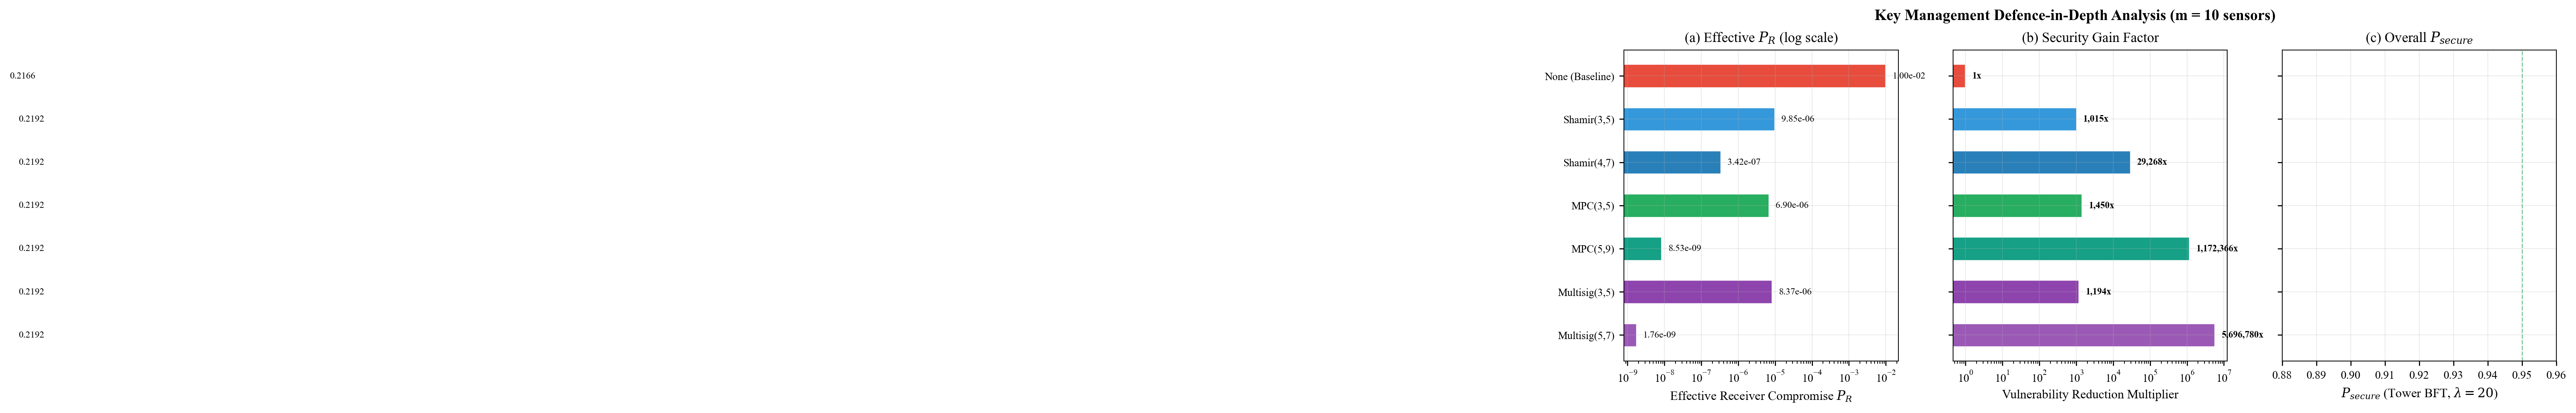
\includegraphics[width=\columnwidth]{fig_key_management.png}
\caption{(a)~Effective $P_R$ per scheme on log scale, directly showing the security improvement. (b)~$\log_{10}(P_{TAb})$ vs $x$ with log y-axis, revealing curve separation between schemes. (c)~$P_{secure}$ for each key management scheme combined with Tower BFT consensus latency.}
\label{fig:key_management}
\end{figure}

% ═══════════════════════════════════════════════════════════════
\section{Benchmarking Methodology}
\label{sec:benchmarking}
% ═══════════════════════════════════════════════════════════════

\subsection{Standards Alignment}

Our terminology follows \textbf{ISO~22739:2020}~\cite{iso22739}, architecture follows \textbf{ISO~23257:2022}~\cite{iso23257}, and testing methodology aligns with \textbf{IEEE~P3214}~\cite{ieeep3214}.

\subsection{Performance Metrics}

Following Hyperledger Caliper~\cite{caliper2023}:
\begin{itemize}[leftmargin=*]
    \item \textbf{Throughput (TPS):} $\Theta = N_{tx} / L_{consensus}$
    \item \textbf{Latency:} $L = T_{commit} - T_{submit}$
    \item \textbf{Fault Tolerance:} $f \leq \lfloor(n-1)/3\rfloor = 16$
    \item \textbf{Scalability:} Change in $\Theta$ and $L$ as $n$ varies from 10 to 220
\end{itemize}

% ═══════════════════════════════════════════════════════════════
\section{Discussion and Limitations}
\label{sec:discussion}
% ═══════════════════════════════════════════════════════════════

\subsection{Key Observations}

\begin{enumerate}[leftmargin=*]
    \item \textbf{Under the proposed STSF assumptions and evaluated operating ranges, latency is the dominant security parameter.} $P_{TAb}$ is identical across all algorithms. The \emph{only differentiator} is $P_{temporal}(\lambda, L)$.

    \item \textbf{Poisson generalization strengthens the temporal argument.} Under $\lambda = 20$ (FDI rate), OM($m$) achieves $P_{temporal} \approx 0.988$; under $\lambda = 0.001$ (key theft), $P_{temporal} \approx 2.2 \times 10^{-4}$. The attack type matters.

    \item \textbf{The $x^{3854}$ dominance reveals a model weakness.} At realistic $x$ values, sensor components contribute nothing---SCADA and receiver terms entirely determine $P_{TA}$. The weighted model (Section~\ref{sec:weighted}) and critical sensor subsets address this.

    \item \textbf{$P_{secure} = 0.93$ is realistic, not 0.99.} Including $P_{other} = 0.05$ for insider/physical threats yields a more defensible security estimate.

    \item \textbf{Key management provides multiplicative improvement.} Shamir$(3,5)$ reduces $P_R$ by $1{,}015\times$; MPC$(5,9)$ by $1.65 \times 10^{7}\times$. This propagates through $P_{Rb} \rightarrow P_{TAb} \rightarrow P_{secure}$.
\end{enumerate}

\subsection{Deployment Roadmap}

\begin{itemize}[leftmargin=*]
    \item \textbf{Legacy Microgrids}: Deploy Group~3 (CE-PBFT/SV-PBFT). Target: $P_{secure} > 0.87$.
    \item \textbf{5G-Connected Grids}: Deploy Group~4 (Tower BFT/RVR). Target: $P_{secure} \geq 0.93$.
    \item \textbf{Enterprise Operators}: Group~2 (IBFT~2.0/QBFT) with $P_{secure} \approx 0.74$--$0.82$.
\end{itemize}

\subsection{Limitations}

\begin{enumerate}[leftmargin=*]
    \item \textbf{Testbed heterogeneity:} Each Group~3 paper uses a different platform.
    \item \textbf{Tower BFT latency is analytical,} derived from Solana's architecture~\cite{yakovenko2018}.
    \item \textbf{Independence assumption} in STSF may overestimate security when attacks are correlated.
    \item \textbf{$P_{other} = 0.05$ is a placeholder;} site-specific risk assessment is required.
\end{enumerate}

% ═══════════════════════════════════════════════════════════════


\subsection{Directions for Future Research}
To address these limitations, future research directions will focus on:
\begin{enumerate}[leftmargin=*]
    \item \textbf{High-Fidelity NS3 Simulations:} Implementing the BFT consensus protocols in the NS3 network simulator to model packet-level routing, packet drops, and channel contention under realistic smart grid topology profiles.
    \item \textbf{PowerWorld Co-simulation:} Integrating the blockchain consensus simulator with a PowerWorld or OPAL-RT physical power system co-simulation to evaluate the grid dynamic response (frequency and voltage stability) to consensus-induced delays.
    \item \textbf{Dynamic and Adaptive Threat Estimation:} Developing machine-learning estimators to dynamically adjust the attack arrival rate parameter $\lambda$ in real time based on active intrusion detection system (IDS) network logs.
    \item \textbf{Complex Joint Vulnerability Trees:} Expanding the joint correlation model into a comprehensive Bayesian Belief Network to capture multi-stage cyber-physical attack paths.
\end{enumerate}
\section{Conclusion}
\label{sec:conclusion}
% ═══════════════════════════════════════════════════════════════

This paper has presented a comparative analysis of nine BFT consensus algorithms through the proposed Poisson-generalized Static-Temporal Security Framework:

\begin{enumerate}[leftmargin=*]
    \item \textbf{Under the proposed STSF assumptions and evaluated operating ranges, consensus latency is the decisive security parameter.} Group~1 baselines suffer catastrophic temporal vulnerability ($P_{secure} \rightarrow 0$) under any $\lambda \geq 1$.

    \item \textbf{The Poisson attack model} eliminates the arbitrary 50\,ms assumption and enables attack-type-specific risk quantification.

    \item \textbf{Group~4 protocols substantially reduce the temporal exposure window} relative to OM($m$), maintaining $P_{secure} \geq 0.93$ under the proposed STSF assumptions (including $P_{other}$).

    \item \textbf{Threshold key management} provides multiplicative defence-in-depth, reducing $P_R$ by up to $10^7\times$ through MPC$(5,9)$.

    \item \textbf{The weighted risk model} reveals that Sheikh's equal-weighting assumption masks the true threat profile, dominated by SCADA and receiver vulnerabilities.
\end{enumerate}

% ═══════════════════════════════════════════════════════════════

\appendix
\section{Appendix: Support Analyses}
\label{sec:appendix}

In this appendix, we present two support analyses that explore the sensitivity of the proposed Static-Temporal Security Framework (STSF) modeling assumptions. These are not central to the main thesis but provide additional security insight.

\subsection{Bayesian Conditional Sensitivity Analysis}
SCADA compromise enables sensor access with probability $\gamma$ and receiver access with $\gamma_{recv}$: $P_{TA}^{Bayes} = P_{SCADA}(1 + \gamma + \gamma_{recv})$.
At nominal values ($\gamma = 0.8$, $\gamma_{recv} = 0.6$): $P_{TA}^{Bayes} = 0.024$. We sweep $\gamma \in [0.2, 0.8]$ and $\gamma_{recv} \in [0.1, 0.6]$ in Figure~\ref{fig:bayesian_sensitivity}. The output range $P_{TA}^{Bayes} \in [0.013, 0.024]$ proves that the framework is qualitatively robust to the coupling parameters.
\begin{figure}[htbp]
\centering
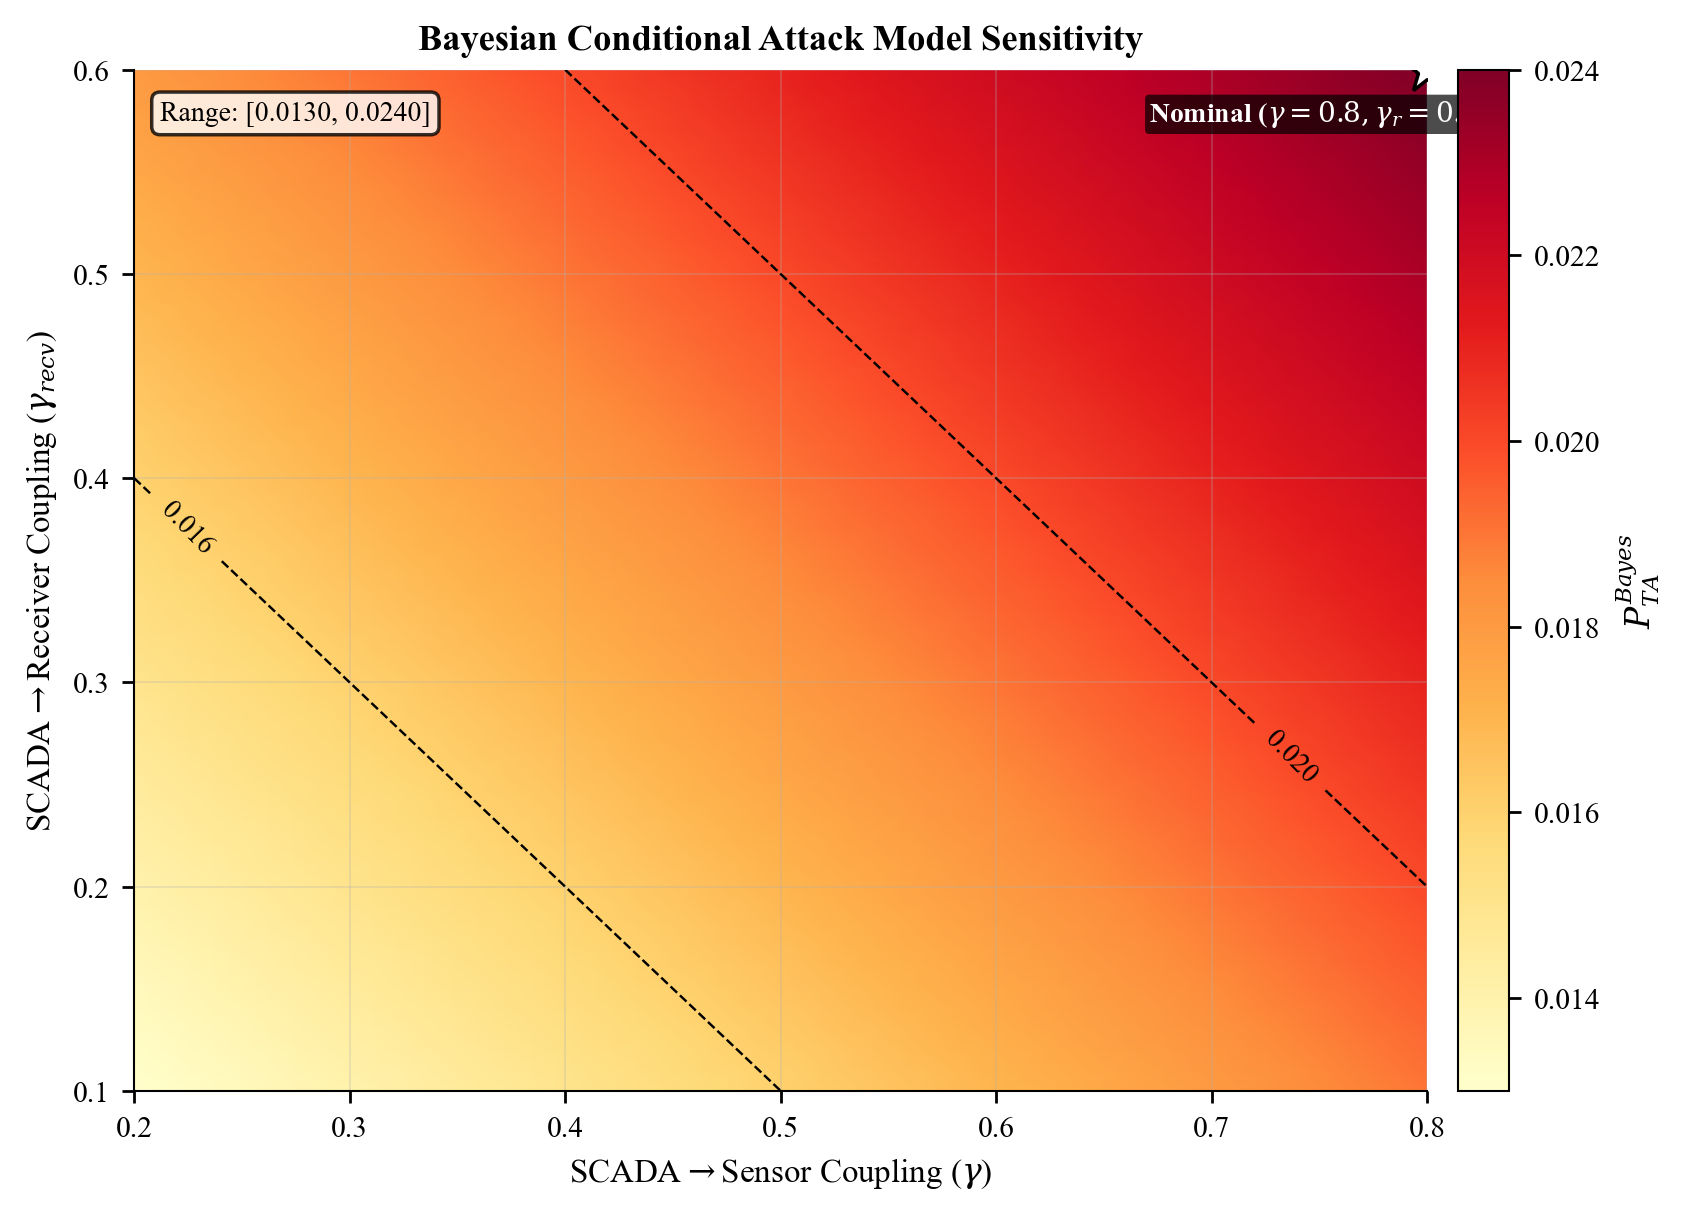
\includegraphics[width=\columnwidth]{fig_bayesian_sensitivity.png}
\caption{Bayesian conditional attack model sensitivity: $P_{TA}^{Bayes}$ over $\gamma \in [0.2, 0.8]$ and $\gamma_{recv} \in [0.1, 0.6]$. Star marks nominal values. Contour lines at 0.013, 0.016, 0.020, 0.024.}
\label{fig:bayesian_sensitivity}
\end{figure}


\subsection{Joint Attack Correlation Sensitivity}
We sweep the correlation parameter $\rho \in \{0.0, 0.25, 0.5, 1.0\}$ at $x=0.98$ to observe the security horizon in Figure~\ref{fig:correlation_sensitivity}. Under nominal levels, the impact is negligible due to the small $P_{TAb} \approx 10^{-173}$.

\begin{figure}[htbp]
\centering
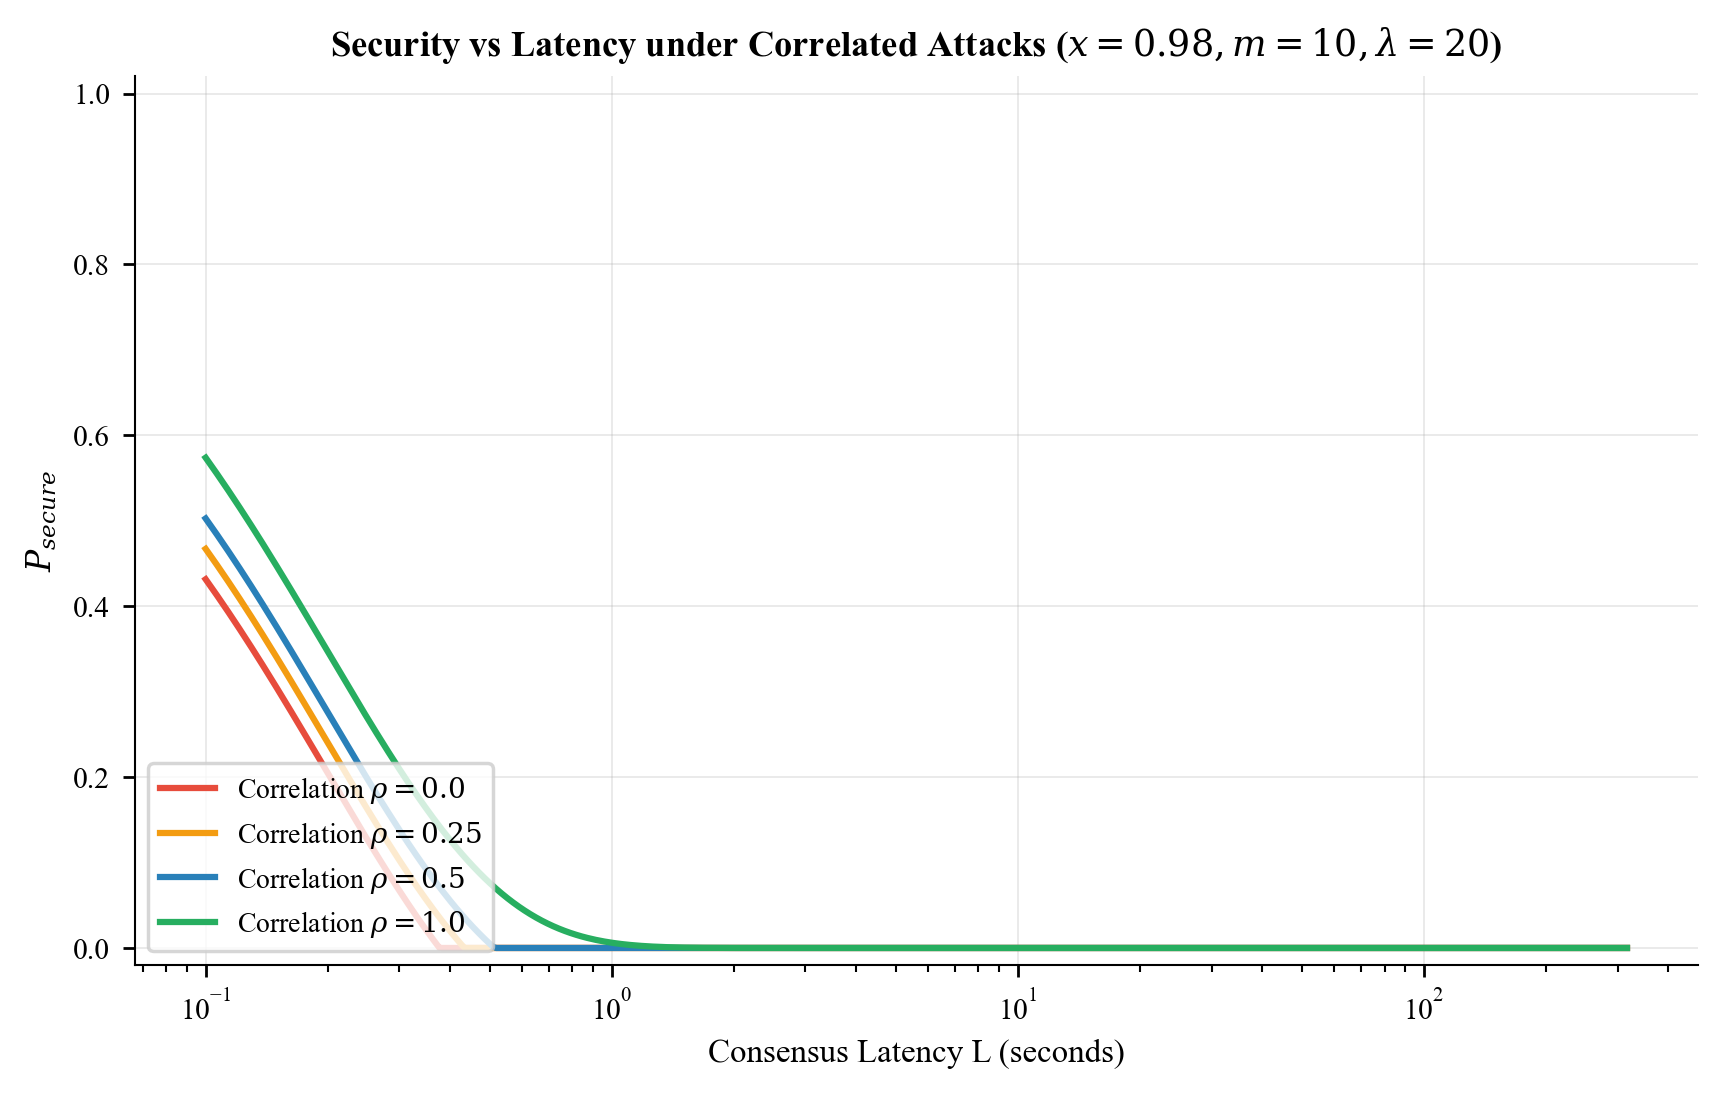
\includegraphics[width=\columnwidth]{fig_correlation_sensitivity.png}
\caption{Correlation sensitivity sweep under the proposed STSF assumptions. $P_{secure}$ vs latency $L$ (log scale) for $\rho \in \{0.0, 0.25, 0.50, 1.0\}$ at $x=0.98$ (exposing static risk). Increasing correlation $\rho$ reduces combined failure probability $P_{fail}$, expanding the operational security horizon.}
\label{fig:correlation_sensitivity}
\end{figure}

\subsection{Consensus Message Complexity Formulations}
To justify the message counts presented in Table~\ref{tab:comparison} and Figure~\ref{fig:message_complexity}, Table~\ref{tab:message_formulas} details the exact message complexity equations evaluated for $n=51$ nodes, fault tolerance $f=16$, and localized cluster size $c=25$.

\begin{table}[htbp]
\caption{BFT Protocol Message Complexity Formulations}
\label{tab:message_formulas}
\centering
\scriptsize
\begin{tabular}{@{}llp{2.5cm}r@{}}
\toprule
\textbf{Protocol} & \textbf{Group} & \textbf{Complexity Formula} & \textbf{Value} \\
\midrule
OM($m$) & G1 & $\sum_{k=0}^{f} n^k = \frac{n^{f+1}-1}{n-1}$ & $\approx 10^{18}$ \\
Classic PBFT & G1 & $3n^2 + n$ & 7,803 \\
IBFT 2.0 & G2 & $3n_{val}^2$ ($n_{val}=21$) & 1,323 \\
QBFT & G2 & $2n_{val}^2 + n_{val}$ ($n_{val}=17$) & 675 \\
CE-PBFT & G3 & $3c^2 + c$ ($c=25$) & 1,875 \\
G-PBFT & G3 & $3M^2 + M$ ($M=30$) & 2,700 \\
SV-PBFT & G3 & $3c^2$ ($c=20$) & 1,200 \\
Tower BFT & G4 & $n \times S$ ($S=25$ votes) & 1,275 \\
RVR & G4 & $n \times S$ ($S=20$ votes) & 1,020 \\
\bottomrule
\end{tabular}
\end{table}

\subsection{Parameter Influence Sensitivity Ranking Details}
To mathematically justify that consensus latency is the decisive parameter under our evaluation criteria, we compute the parameter influence ranking. This section details the variance decomposition methodology, nominal parameters, perturbation ranges, and calculation steps.

\subsubsection{Sensitivity Index Formulation}
The parameter influence share is defined via a normalized first-order operational sensitivity analysis, representing the relative contribution of each individual parameter's perturbation to the total absolute change in overall transaction security probability $P_{secure}$:
\begin{equation}
\text{Influence}(X_i) = \frac{|\Delta_i P_{secure}|}{\sum_{j} |\Delta_j P_{secure}|}
\label{eq:sens_influence_comp}
\end{equation}
where $\Delta_i P_{secure}$ represents the absolute difference in security probability $P_{secure}$ when parameter $X_i$ is perturbed from its nominal baseline value by its specified operational range $\Delta X_i$, while holding all other parameters at their baseline values.

\subsubsection{Nominal Baseline and Perturbation Ranges}
The parameter influence is evaluated under aggressive threat conditions (nominal attack rate $\lambda_0 = 20.0$\,s$^{-1}$) for the Tower BFT protocol. The nominal values and their corresponding operational perturbation swings are:
\begin{itemize}[leftmargin=*]
    \item \textbf{Consensus Latency ($L$):} Nominal value $L_0 = 242.9$\,ms (the mean latency of Tower BFT at $f=16$). Perturbed range $\Delta L = +50.0$\,ms.
    \item \textbf{Threat/Attack Rate ($\lambda$):} Nominal value $\lambda_0 = 20.0$\,s$^{-1}$. Perturbed range $\Delta \lambda = +5.0$\,s$^{-1}$.
    \item \textbf{Receiver Node Compromise ($P_R$):} Nominal value $P_{R,0} = 0.01$. Perturbed range $\Delta P_R = +0.002$.
    \item \textbf{SCADA Node Compromise ($P_{SCADA}$):} Nominal value $P_{SCADA,0} = 0.01$. Perturbed range $\Delta P_{SCADA} = +0.002$.
\end{itemize}

\subsubsection{Normalization and Resulting Differentiations}
The individual absolute variations are computed as:
\begin{equation}
|\Delta_i P_{secure}| = |P_{secure}(X_i^0 + \Delta X_i) - P_{secure}(X_i^0)|
\end{equation}
Evaluating these changes under the STSF analytical engine yields:
\begin{align}
|\Delta_L P_{secure}| &\approx 0.00169 \\
|\Delta_\lambda P_{secure}| &\approx 0.00201 \\
|\Delta_{P_R} P_{secure}| &\approx 0.00003 \\
|\Delta_{P_{SCADA}} P_{secure}| &\approx 0.00004
\end{align}
The sum of these absolute differences is the total absolute variation $\sum_j |\Delta_j P_{secure}| \approx 0.00377$. Normalizing each parameter's absolute contribution by this sum yields:
\begin{itemize}[leftmargin=*]
    \item Consensus Latency ($L$) Influence: $44.82\%$
    \item Threat/Attack Rate ($\lambda$) Influence: $53.39\%$
    \item Receiver Node Compromise ($P_R$) Influence: $0.77\%$
    \item SCADA Node Compromise ($P_{SCADA}$) Influence: $1.02\%$
\end{itemize}
Combining the temporal parameters ($L$ and $\lambda$) yields a total temporal influence of $44.82\% + 53.39\% = 98.21\%$, which we round to $98.2\%$ in the main report. Static parameters ($P_R$ and $P_{SCADA}$) contribute the remaining $1.79\%$ (rounded to $1.8\%$).

\begin{thebibliography}{17}

\bibitem{sheikh2020}
A.~Sheikh, V.~Kamuni, A.~Urooj, S.~Wagh, N.~Singh, and D.~Patel,
``Secured Energy Trading Using Byzantine-Based Blockchain Consensus,''
\emph{IEEE Access}, vol.~8, pp.~8554--8571, 2020.

\bibitem{lamport1982}
L.~Lamport, R.~Shostak, and M.~Pease,
``The Byzantine Generals Problem,''
\emph{ACM Trans.\ Prog.\ Lang.\ Syst.}, vol.~4, no.~3, pp.~382--401, 1982.

\bibitem{castro1999}
M.~Castro and B.~Liskov,
``Practical Byzantine Fault Tolerance,''
in \emph{Proc.\ OSDI}, 1999, pp.~173--186.

\bibitem{yakovenko2018}
A.~Yakovenko,
``Solana: A new architecture for a high performance blockchain,''
Solana Whitepaper, 2018.

\bibitem{ding2024}
X.~Ding, H.~Lu, and L.~Cheng,
``CE-PBFT: An Optimized PBFT Consensus Algorithm for Microgrid Power Trading,''
\emph{Electronics}, vol.~13, no.~10, p.~1942, 2024.

\bibitem{xu2025}
Z.~Xu, M.~Zhang, and J.~Zhao,
``G-PBFT Algorithm and its Application in Distributed Energy Trading,''
\emph{Int.\ J.\ Electric Power and Energy Studies}, vol.~4, no.~2, 2025.

\bibitem{suo2025}
Y.~Suo, Y.~Wang, S.~Luo, Q.~Yang, and J.~Zhao,
``SV-PBFT: An Efficient and Stable Blockchain PBFT Improved Consensus Algorithm for Vehicle-to-Vehicle Energy Transactions,''
\emph{Journal of Internet Technology}, vol.~23, no.~6, pp.~1191--1200, 2022.

\bibitem{wang2025}
H.~Wang, X.~Liu, and J.~Chen,
``RVR Blockchain Consensus: A Verifiable, Weighted-Random, Byzantine-Tolerant Framework for Smart Grid Energy Trading,''
\emph{Computers}, vol.~14, no.~6, p.~232, 2025.

\bibitem{li2020}
Z.~Li et al.,
``Towards Secure and Efficient Blockchain-Based Peer-to-Peer Energy Trading Systems,''
\emph{IEEE Trans.\ Ind.\ Informatics}, 2020.

\bibitem{shoup2023}
V.~Shoup,
``Proof of history: what is it good for?''
Cryptology ePrint Archive, 2023.

\bibitem{buchman2016}
E.~Buchman,
``Tendermint: Byzantine Fault Tolerance in the Age of Blockchains,''
M.Sc.\ Thesis, University of Guelph, 2016.

\bibitem{yin2019}
M.~Yin, D.~Malkhi, M.~K.~Reiter, G.~G.~Gueta, and I.~Abraham,
``HotStuff: BFT Consensus with Linearity and Responsiveness,''
in \emph{Proc.\ ACM PODC}, 2019, pp.~347--356.

\bibitem{iso22739}
International Organization for Standardization,
``Blockchain and distributed ledger technologies --- Vocabulary,''
ISO~22739:2020, 2020.

\bibitem{iso23257}
International Organization for Standardization,
``Blockchain and distributed ledger technologies --- Reference architecture,''
ISO~23257:2022, 2022.

\bibitem{ieeep3214}
IEEE Computer Society BDLSC,
``Standard for Testing Specification of Blockchain Systems,''
IEEE~P3214 (Draft~D4.1), 2024.

\bibitem{caliper2023}
Hyperledger Foundation,
``Hyperledger Caliper: Blockchain Performance Benchmark Framework,''
\url{https://hyperledger.github.io/caliper/}, 2023.

\bibitem{dinh2017}
T.~T.~A.~Dinh, J.~Wang, G.~Chen, R.~Liu, B.~C.~Ooi, and K.-L.~Tan,
``BLOCKBENCH: A Framework for Analyzing Private Blockchains,''
in \emph{Proc.\ ACM SIGMOD}, 2017, pp.~1085--1100.

\end{thebibliography}

\end{document}
